
\documentclass{mproj}
\usepackage{graphicx}

\usepackage{url}
\usepackage{fancyvrb}
\usepackage[final]{pdfpages}
\usepackage{times}

%\usepackage[nottoc,numbib]{tocbibind}
\usepackage[nottoc]{tocbibind}

% for alternative page numbering use the following package
% and see documentation for commands
%\usepackage{fancyheadings}


% other potentially useful packages
%\uspackage{amssymb,amsmath}
%\usepackage{url}
%\usepackage{fancyvrb}
%\usepackage[final]{pdfpages}

% \usepackage{CTEX} % 中文支持
\usepackage{comment}

\usepackage[section]{placeins}  % 添加这个以限制浮动体跨越节的边界

\usepackage{listings}
\lstset{
    basicstyle=\normalfont,
    breaklines=true
}
\usepackage{xcolor} % 用于定义颜色

\usepackage{amsmath}

\usepackage{hyperref}
\usepackage{cleveref}
\crefname{figure}{Figure}{Figures} % 设置 \cref 引用图像的格式
\crefname{appendix}{Appendix}{Appendices}
\crefname{section}{Section}{Sections}
\crefname{equation}{Equation}{Equations}
\crefname{chapter}{Chapter}{Chapters}

\begin{document}

%%%%%%%%%%%%%%%%%%%%%%%%%%%%%%%%%%%%%%%%%%%%%%%%%%%%%%%%%%%%%%%%%%%
%Towards Faster Parallelism: Performance-Driven Workstealing Scheduling in YewPar
\title{Towards Faster Combinatorial Search: Performance-Driven Workstealing Policy in YewPar}
\author{Hao Xie}
\date{31th August 2023}
\maketitle
%%%%%%%%%%%%%%%%%%%%%%%%%%%%%%%%%%%%%%%%%%%%%%%%%%%%%%%%%%%%%%%%%%%

%%%%%%%%%%%%%%%%%%%%%%%%%%%%%%%%%%%%%%%%%%%%%%%%%%%%%%%%%%%%%%%%%%%
\begin{abstract}

    Precise combinatorial search is indispensable for a wide range of applications,
    including constraint programming, graph matching, and computational algebra.
    Parallel computation serves as one of the vital means to accelerate combinatorial search.
    Workstealing stands as a crucial strategy for achieving parallel computation,
    where idle computational resources of a node exploit the residual tasks from other nodes,
    enhancing the overall performance.
    YewPar is an exemplary parallel framework tailored for combinatorial search.
    It offers an array of robust skeletons and policies, enabling developers to effortlessly parallelize their search algorithms.
    However, its workstealing strategy leans towards randomly selecting task-rich nodes for task theft,
    often leading to unnecessary overhead and latency.
    Our objective is to boost the execution speed of applications based on the YewPar framework by designing a novel workstealing strategy.

    To this end, we devised and implemented a new framework termed "Performance-Driven Workstealing Policy",
    which dynamically adjusts the target node for task theft based on multiple performance parameters of each node.
    The core philosophy of this framework revolves around various strategies,
    such as stealing tasks from nodes with higher loads to approximate a load-balanced state,
    thereby shortening the time taken by the last worker to complete its task.
    By reducing unnecessary probing durations, the starvation time for workers without tasks is minimized,
    ultimately curtailing the total execution time of applications based on YewPar under parallel conditions.

    Furthermore, we evaluated the enhanced YewPar with the improved Workstealing strategy.
    The assessment was conducted on a Beowulf cluster equipped with multi-core machines.
    The results indicate that the revamped YewPar, compared to its original version,
    achieves superior performance across varying node counts and workloads.
    Without compromising the search results, it can significantly reduce the execution time of search applications based on YewPar.
    In most scenarios, the improvements in its execution speed are quite remarkable.

    \textbf{Keywords:} Combinatorial Search, Parallel Computation, Workstealing, YewPar, Performance-Driven Policy, Beowulf Cluster.

\end{abstract}
%%%%%%%%%%%%%%%%%%%%%%%%%%%%%%%%%%%%%%%%%%%%%%%%%%%%%%%%%%%%%%%%%%%

%%%%%%%%%%%%%%%%%%%%%%%%%%%%%%%%%%%%%%%%%%%%%%%%%%%%%%%%%%%%%%%%%%%
\educationalconsent


%%%%%%%%%%%%%%%%%%%%%%%%%%%%%%%%%%%%%%%%%%%%%%%%%%%%%%%%%%%%%%%%%%%

\newpage
%%%%%%%%%%%%%%%%%%%%%%%%%%%%%%%%%%%%%%%%%%%%%%%%%%%%%%%%%%%%%%%%%%%
\section*{Acknowledgements}

It took months almost entirely to focus on this project and do this dissertation.
As a student unfamiliar with the topic initially,
I have done much work with effort and interest to gain knowledge regarding the YewPar framework,
Combinatorial Search and Workstealing concepts related to the project.

So, I would like to thank my supervisor Blair Archibald, who helped me a lot in completing this project.
He discussed the project with me every week and gave me a lot of advice, which benefited me
greatly.

I would also like to thank my family for their love and support throughout my life. Also, my
roommates and other friends, who encouraged me a lot during my project.

%%%%%%%%%%%%%%%%%%%%%%%%%%%%%%%%%%%%%%%%%%%%%%%%%%%%%%%%%%%%%%%%%%%
\tableofcontents
%%%%%%%%%%%%%%%%%%%%%%%%%%%%%%%%%%%%%%%%%%%%%%%%%%%%%%%%%%%%%%%%%%%

%%%%%%%%%%%%%%%%%%%%%%%%%%%%%%%%%%%%%%%%%%%%%%%%%%%%%%%%%%%%%%%%%%%
\chapter{Introduction}\label{intro}

Precise combinatorial search is essential for a broad spectrum of applications,
including constraint programming, graph matching, and computational algebra.
Combinatorial problems are addressed by systematically exploring the search space,
a process both theoretically and practically computationally challenging.
Exact search, in particular, traverses the entire search space to offer a provably optimal solution.
Conceptually, exact combinatorial search operates by generating and navigating through a (massive) tree representing potential solutions.
Incorporating parallelism, on-the-fly tree generation, search heuristics, and pruning can diminish the execution time of an exact search.
Due to the vast and highly irregular search trees, parallelizing exact combinatorial search poses significant challenges.

A framework known as YewPar\cite{10.1145/3332466.3374537} stands out as the first scalable parallel framework tailored for precise combinatorial search.
YewPar aims to allow non-specialist users to benefit from parallelism,
reuse parallel search patterns encoded as algorithmic skeletons,
and execute across diverse parallel architectures.

Concurrently, with the proliferation of parallel computing and multi-core processors, effective task scheduling becomes increasingly paramount.
A key feature of YewPar is its capability to parallelize search, accomplished by allowing multiple workers in a node to steal tasks from other nodes' task pools when their local task pools run dry.
In YewPar, when a local task pool is empty, it randomly selects nodes for task theft.
Workstealing, a widely researched and implemented parallel scheduling strategy, permits idle processors to "steal" tasks from their busier counterparts.
However, many internal Workstealing schedulers, like YewPar, tend to adopt a somewhat random theft approach, often leading to unnecessary overhead, latency, and a vast amount of time spent in probing for tasks to steal.
This often results in relative load imbalances across nodes, prolonging the overall completion time.
While numerous improvements on Workstealing have emerged, many fail to adequately balance features such as lightweight design, decentralization, high performance, and generalizability.

Our objective is to enhance YewPar's performance by refining its Workstealing strategy.
To this end, this paper introduces a new "Performance-Driven Workstealing Policy" framework.
Its core philosophy centers on attempting to steal tasks from higher-load nodes to approximate a balanced load state, thereby reducing the time taken for the last worker to complete its task.
Additionally, by minimizing unnecessary task probing and theft durations, the starvation time for task-less workers is reduced,
ultimately shortening the runtime of YewPar-based applications in a parallel environment.

This framework boasts multiple features:
it periodically monitors and transmits valuable data,
calculates and caches the optimal node for task theft,
and efficiently gathers and shares multiple performance metrics, such as node load status, remaining tasks per node, and inter-node communication latency, at a low cost using proprietary architecture and data processing algorithms.
Through its in-house "Time-Optimized Workstealing Strategy" algorithm, it calculates the optimal theft node and caches it, refreshing periodically.
Idle workers, if they fail to obtain tasks from the cached target, initiate an auxiliary refresh operation, assisting potential dormant refreshers in refreshing the optimal theft target cache.
Collectively, these components enable the acceleration effects of the Performance-Driven Workstealing Policy.

Furthermore, we evaluated the YewPar enhanced with the refined Workstealing strategy.
Assessments were conducted on a Beowulf cluster equipped with multi-core machines.
Results revealed that the improved YewPar, under varying node counts and workloads, outperforms the original YewPar in terms of performance.
Without compromising the search results, it can significantly reduce the execution time of search applications based on YewPar.
In most scenarios, the improvements in its execution speed are quite pronounced.

%%%%%%%%%%%%%%%%%%%%%%%%%%%%%%%%%%%%%%%%%%%%%%%%%%%%%%%%%%%%%%%%%%%
\chapter{Background}\label{survey}

\section{Modern Strategies in Distributed Concurrency}
\subsection{Workstealing}

Workstealing is a core concept in parallel programming.
Its primary advantage lies in decentralized scheduling,
where each processor autonomously manages its task queue,
significantly reducing the overhead brought about by global synchronization.
The idea of Workstealing can be traced back to the implementation of the Multilisp programming language in the 1980s and the work on parallel functional programming languages\cite{10.1145/324133.324234}.
It has been employed in the scheduler of the Cilk programming language\cite{BLUMOFE199655},
Java's fork/join framework\cite{lea2000forkjoin},
.NET's Task Parallel Library\cite{leijen2009design},
and Rust's Tokio runtime\cite{tokio,krill2021tokio},
among many other parallel frameworks and libraries.

\begin{figure}[h]
    \centering
    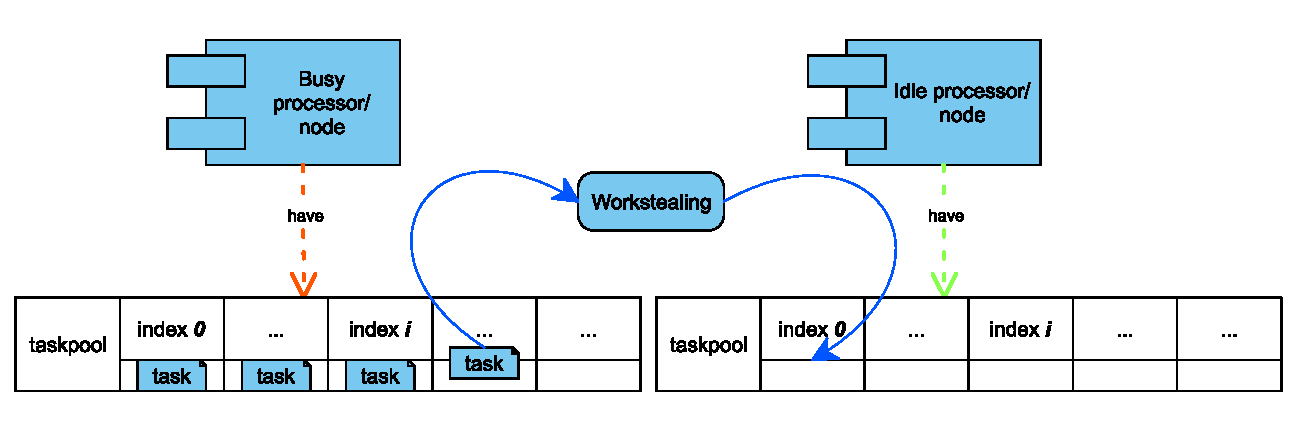
\includegraphics[width=0.98\textwidth]{images/workstealing.pdf}
    \caption{Workstealing example}
    \label{fig:workstealing}
\end{figure}
\FloatBarrier

As illustrated in \cref{fig:workstealing},
in the workstealing strategy, every processor within the system possesses its own queue of tasks awaiting execution.
Each task consists of a series of instructions that need to be executed sequentially.
During execution, a task might spawn new sub-tasks.
These sub-tasks are preliminarily placed in the queue of the processor executing the parent task.
When a processor's task queue becomes empty, it attempts to "steal" tasks from other processors' queues.
Thus, Workstealing essentially schedules tasks to idle processors,
ensuring that scheduling overhead only occurs when all processors are occupied\cite{10.1145/1248377.1248396}.

In contrast to Workstealing stands the work-sharing strategy,
another approach to dynamic multithreading scheduling.
In work-sharing, newly generated tasks are immediately scheduled on a processor for execution.
Compared to this, Workstealing reduces task migration between processors,
as such migration doesn't occur when all processors are busy\cite{10.1145/324133.324234}.

Algorithms like the randomized Workstealing algorithm proposed by Blumofe and Leiserson maintain multiple execution threads (asynchronous tasks) and schedule them on PP processors\cite{10.1145/324133.324234}.
Each processor has a double-ended queue (deque) for storing threads,
designating the two ends as "top" and "bottom".
When a processor has a current thread to execute,
it processes the instructions in the thread sequentially until encountering one of four "special" behaviors:
\begin{itemize}
    \item A "spawn" instruction creates a new thread. The current thread is placed at the bottom of the deque, and the processor starts executing the new thread.
    \item A "stall" instruction temporarily halts the execution of its thread. The processor pops a thread from the bottom of its deque and starts its execution. If its deque is empty, it initiates workstealing.
    \item Some instructions might terminate a thread. The behavior in this case is the same as a stalling instruction.
    \item An instruction might activate another thread. The other thread is pushed to the bottom of the deque, but the processor continues executing its current thread.
\end{itemize}
Initially, a computation comprises a single thread assigned to a processor, while other processors start off idle.
Any idle processor commences the actual Workstealing process, involving the following steps:
\begin{itemize}
    \item It randomly picks another processor.
    \item If the other processor's deque is non-empty, it pops the topmost thread from the deque and begins its execution;
    \item Otherwise, the process is repeated.
\end{itemize}

However, strategies like this random theft often incur considerable overhead in complex multi-node environments.
Such overhead primarily originates from the "thief" randomly probing nodes in the cluster to locate a "victim".
Given the uneven distribution of cluster scales, this problem becomes more pronounced,
resulting in excessive system messaging and prolonged starvation periods for "thieves" due to multiple theft failures and network latencies.
While optimization attempts concerning Workstealing have never ceased,
such as establishing fixed "matchmaker" nodes and notifying them of the current states of nodes with excess tasks and those without,
to enable "matchmaker" nodes to match task-starved nodes with those abundant in tasks\cite{10.1145/2851141.2851175},
the maintenance of these "matchmaker" nodes and the waiting time for sending query requests to them during task starvation remain significant overheads.
Additionally, they only match nodes with extra tasks to those without,
without optimizing based on various performance parameters of the nodes,
which might lead to frequent unnecessary thefts.
Strategies specifically designed for Multicore Event-Driven Systems\cite{5541655},
though considering the characteristics of event-driven programming and effectively increasing parallelism in such environments,
still introduce additional overhead through task randomization and delayed theft strategies and might not be well-suited for non-event-driven applications.

To date, no strategy has emerged as a universally efficient, low-overhead, lightweight, cross-platform solution.
Workstealing remains primarily in the phase of targeted optimization for various application environments.
Our task theft scheme design, based on node performance data, mainly employs performance data such as worker load conditions, remaining tasks of each node, and communication delays between nodes.
This data can be effortlessly acquired in other frameworks employing the Workstealing strategy,
ensuring excellent portability and universality.
It can be easily ported to platforms and frameworks other than YewPar, and the design also possesses lightweight characteristics.

\subsection{The Pitfalls of Locking Mechanisms and the Promise of Lock-Free Designs}\label{survey_lock}

Optimization in multithreading is a burgeoning field,
where locking mechanisms have been primarily designed to address inconsistencies in concurrent operations.
Edward A. Lee once posited that lock mechanisms are among the primary issues in multithreading\cite{1631937}.
Locks can induce thread waiting, leading to performance degradation.
In high-concurrency scenarios, such waiting can manifest as severe performance bottlenecks.
Furthermore, when multiple threads vie for the same lock, they enter a state of contention.
Such a state not only diminishes performance but can also induce thread starvation,
wherein certain threads may perpetually be denied lock access.
Lee emphasized that while various techniques can alleviate these issues,
the ultimate solution lies in seeking alternative programming methodologies and models to multithreading,
with lock-free programming emerging as a promising avenue.

Currently, there are numerous exemplary implementations of lock-free designs.
For instance, there exists a lock-free concurrent queue algorithm that facilitates multiple threads to access
and modify the queue concurrently without necessitating locks\cite{10.1145/248052.248106}.
Moreover, a dynamic hash table design based on a lock-free paradigm has been introduced.
Owing to the elimination of lock overheads, this design offers stellar performance in high-concurrency settings\cite{10.1145/564870.564881}.

This paper draws inspiration from various lock-free designs,
introducing lock-free data structures and algorithms.
Our Performance-Driven Workstealing Policy framework, while ensuring data accuracy,
circumvents the performance implications of locks.
To a certain extent, this ensures the framework's lightweight nature and high performance.

\section{Combinatorial Search}
In computer science and artificial intelligence, combinatorial search refers to a method employed
to find solutions within a designated search space.
Classic combinatorial search challenges encompass problems like the Eight Queens puzzle and
assessing actions in games with extensive game trees, such as Othello or Chess.
This type of search is particularly apt for problems where the solution space is vast,
making it infeasible to enumerate all possible solutions.
Certain algorithms guarantee the discovery of the optimal solution,
while others may only yield the best solution found within the explored state space.
Through branch and bound techniques or by adopting heuristic approaches,
combinatorial search can effectively reduce the search space, facilitating a swifter solution discovery.

\subsection{Parallel Combinatorial Search and YewPar}
With the evolution of modern computer hardware, especially the proliferation of multi-core processors
and distributed systems, leveraging parallelism to expedite combinatorial search has emerged as a research hotspot.
The aim of parallel combinatorial search is to decompose the search space into multiple segments,
enabling concurrent execution across various processing units, thereby accelerating solution discovery.

Parallel tree search can be categorized\cite{gendron1994parallel} as follows:
\begin{enumerate}
    \item Parallel Node Processing focuses on parallelizing branching/boundary operations,
          as illustrated by boundary calculations for the Flowshop problem on GPUs\cite{gmys2016work}.
    \item Space partitioning, where parallel workers speculatively explore subtrees of the search tree.
          Even though subtrees are explored independently, knowledge such as improved boundaries is typically
          shared amongst workers to enhance performance.
    \item Combinatorial methods run competitive searches in parallel, usually employing diverse heuristics
          or boundary approaches. Hybrid methods combining these strategies are also employed.
\end{enumerate}

\begin{figure}[h]
    \centering
    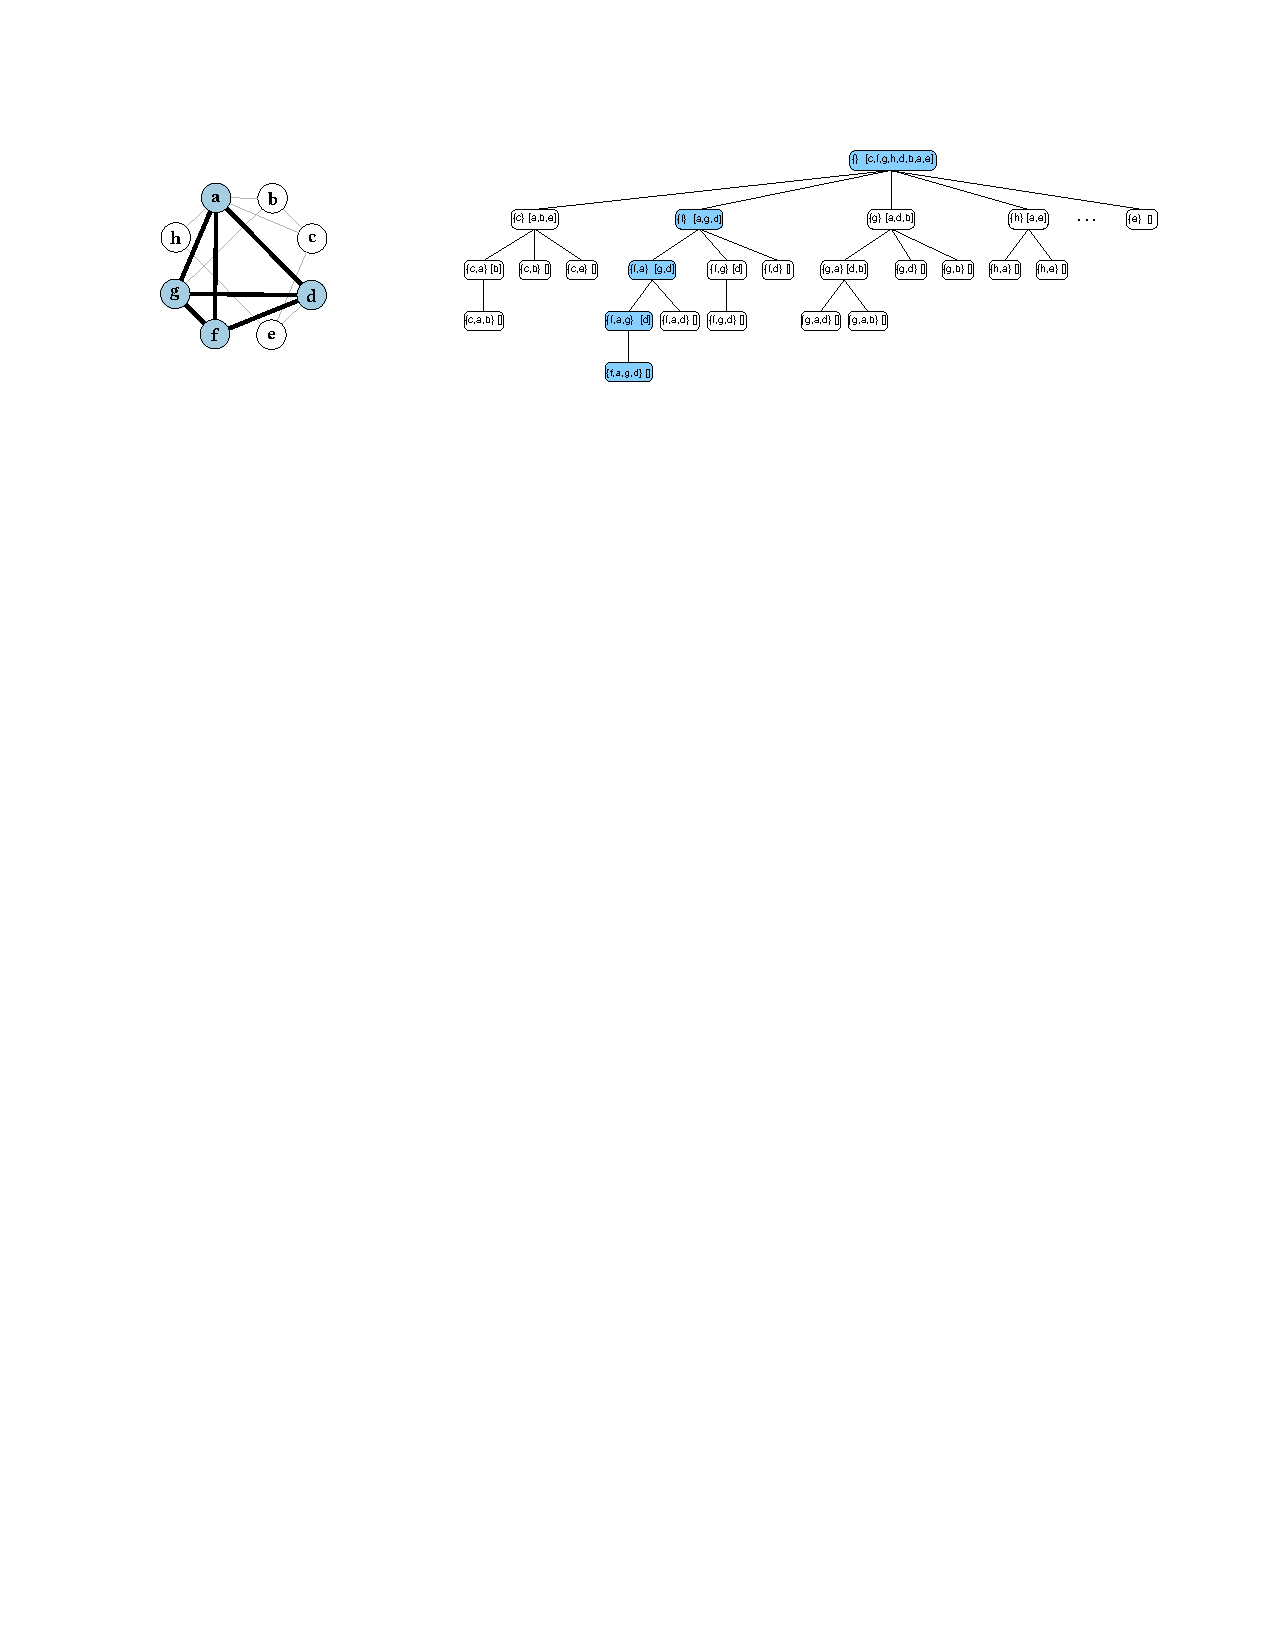
\includegraphics[width=0.98\textwidth]{images/yewpar_maxclique.pdf}
    \caption{Maximum clique instance in YewPar. Input graph with clique \{a,d,f,g\} to the left and corresponding search tree to the right. Each tree node displays the current clique and a list of candidate vertices (in heuristic order) to extend that clique. Reproduced from \cite{10.1145/3332466.3374537}}
    \label{fig:yewpar_maxclique}
\end{figure}
\FloatBarrier

YewPar stands as a parallel framework explicitly designed for combinatorial search.
It offers a suite of robust tools and strategies, allowing developers to effortlessly parallelize their search algorithms.
YewPar's primary attributes are its flexibility and scalability,
equipping it to handle a wide range of intricate search scenarios.
Within YewPar, work-stealing serves as the central strategy for task scheduling,
enabling processors to steal tasks from others when their local task queues are empty.
This ensures all processors remain occupied, thereby optimizing overall performance.

\subsubsection{Performance Anomalies}
\label{sec:performance_anomalies}
Search algorithms rely on sorting heuristics to swiftly identify useful nodes,
such as target nodes in decision problems
or a strongly constrained node in branch and bound optimization problems.
To capitalize on these heuristics,
searches proceed in a left-to-right order (across all tree depths).
Therefore, a sequential search has complete information about the search tree,
obtaining insights from all nodes on its left, and the search remains deterministic.
Parallel search tentatively explores subtrees without the full left-side information and
might benefit from a right-to-left information flow.
However, this speculation implies that parallel searches might undertake more work
than their sequential counterparts.
Consequently, parallel searches are notoriously recognized for performance anomalies\cite{10.1007/3-540-60321-2_29}.
Detrimental anomalies occur when the runtime on \( w \) worker threads surpasses that on \( w-1 \) threads.
Here, the extra work might outweigh the benefits of added computational resources,
or the additional computational resources might disrupt the search heuristics.
Acceleration anomalies signify super-linear acceleration,
often attributed to the information flow from right to left,
which allows for more pruning than in sequential searches, thereby reducing the overall workload.
The presence of anomalies complicates the parallel performance prediction for speculative search applications.
Yew-Par aims to avoid detrimental anomalies while permitting acceleration anomalies;
\cite{ARCHIBALD201892} reports a specialized search framework that carefully controls anomalies
to offer replicable performance guarantees.

\subsection{The Rationale for Designing and Employing a Novel Workstealing Strategy in YewPar}
YewPar employs Workstealing as its pivotal distributed parallelization scheduling strategy,
but it utilizes a biased random stealing approach\cite{archibald2019yewpar}.
Idle workers attempt to steal tasks from other nodes randomly until they secure a valid task,
then lock onto that node for stealing until they can no longer pilfer tasks from it.
Only then do they randomly select another node for theft.
This method might induce unnecessary overheads and idle computational resources,
especially amidst uneven task distributions and when nodes possess imbalanced computational assets.
Given the characteristics of combinatorial searches,
there might be a vast disparity in the number of tasks across nodes and
a significant execution time variance between tasks.
This suggests that the random stealing approach is more likely to yield prolonged starvation times for idle workers,
rendering it a suboptimal choice.

For optimal utilization of computational capabilities across node cores and to curtail redundant communication overheads,
YewPar necessitates a more intelligent Workstealing strategy.
The proposed Performance-Driven Workstealing Policy, tailored to node performance,
addresses this issue.
By economically evaluating each node's performance, such as the average task execution time,
this new strategy employs a stealing algorithm designed around performance parameters
to precisely and dynamically update the optimal stealing target, thereby enhancing overall performance.


%%%%%%%%%%%%%%%%%%%%%%%%%%%%%%%%%%%%%%%%%%%%%%%%%%%%%%%%%%%%%%%%%%%
\chapter{Design and implementation}\label{design}

\section{Overall Design}

The Performance-Driven Workstealing Policy framework designed in this study encompasses:
\begin{itemize}
    \item Scheduler Channel: Primarily responsible for monitoring, gathering statistics,
          and transmitting the load status of all workers within the node.
    \item Performance Monitor: Primarily tasked with collecting various performance data,
          transmitting processed local performance metrics, and computing and caching the ID of
          the optimal node for task stealing.
    \item Performance Policy: Mainly engaged in obtaining the optimal stealing target from
          the Performance Monitor when the local task pool is empty.
\end{itemize}

The relationship between these components is depicted in \cref{fig:overall_architecture}.
\begin{figure}[h]
    \centering
    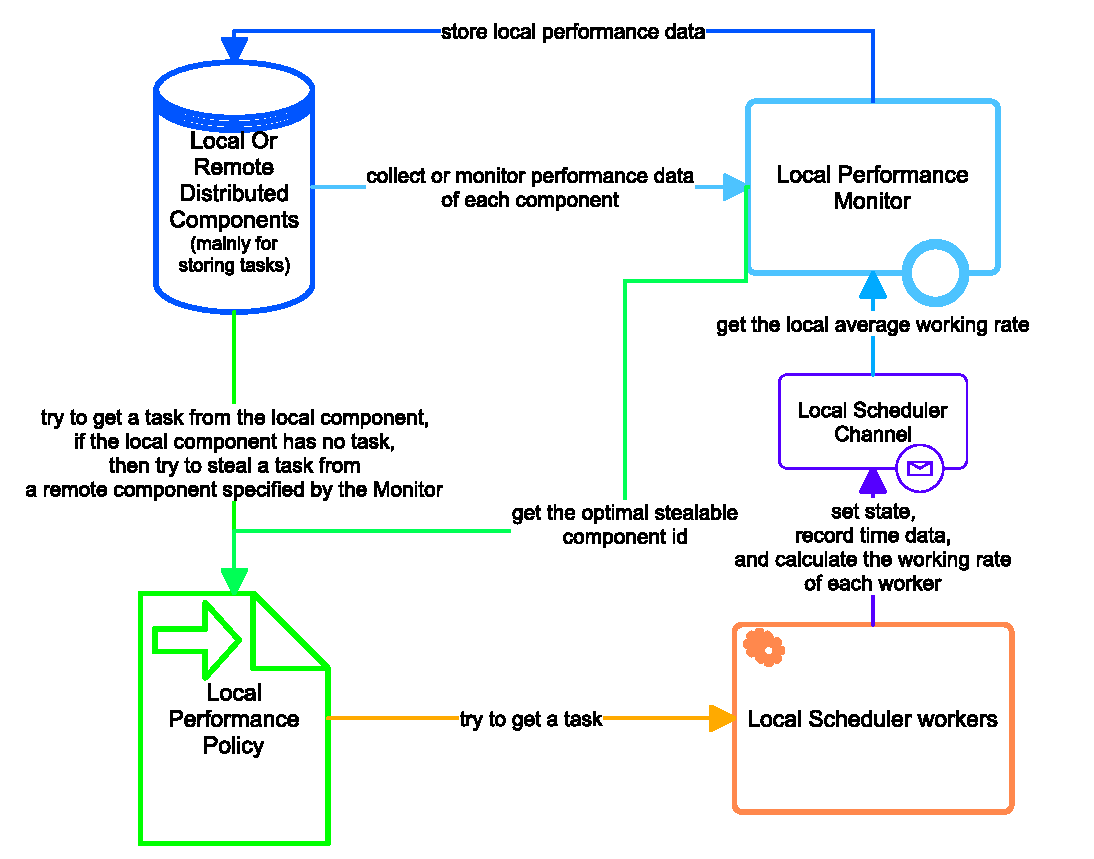
\includegraphics[width=0.9\textwidth]{images/overall_architecture.pdf}
    \caption{Performance-Driven Workstealing Policy Architecture}
    \label{fig:overall_architecture}
\end{figure}
\FloatBarrier

Among them, the Performance Monitor chiefly handles the gathering and transmission of performance metrics
and calculates and caches the ID of the optimal node for task stealing.
The distributed component is responsible for storing task pools and performance data
accessible both remotely and locally, offering access and modification operations through the HPX framework's action.
The Scheduler Channel provides an interface allowing workers to update their current load status
and compute their load data. Workers are tasked with obtaining executable tasks from the Performance Policy.
Meanwhile, the Performance Policy is charged with drawing tasks from the local task pool
or, after obtaining the optimal stealing target node from the Performance Monitor, stealing tasks from its task pool.

%%%%%%%%%%%%%%%%%%%%%%%%%%%%%%%%%%%%%%%%%%%%%%%%%%%%%%%%%%%%%%%%%%%

\section{Performance Data Collection and Transmission}
Data collection encompasses three aspects: load status across nodes,
remaining task volume on each node,
and the time each node takes to retrieve tasks from the task pool.
These parameters will provide robust data support for subsequent optimal stealing target calculations.
Furthermore, to ensure the collection of more effective data at a lower cost,
this paper meticulously designs and optimizes all three aspects.

\subsection{Load Status of All Workers on a Node}
Initially, the YewPar's System Stack appears as illustrated in
\cref{fig:yewpar_system_stack}
\cite{10.1007/978-3-030-29400-7_14}.

\begin{figure}[h]
    \centering
    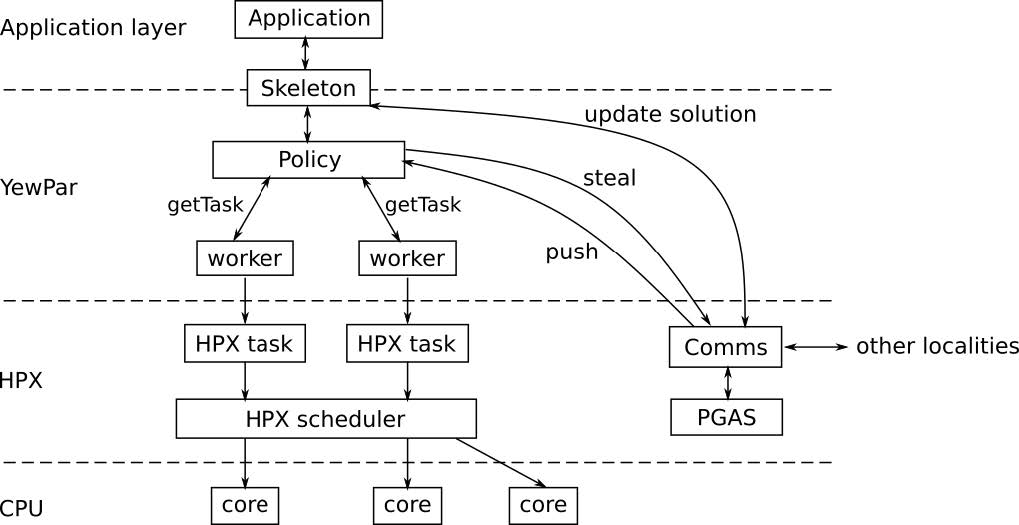
\includegraphics[width=0.9\textwidth]{images/YewPar_System_Stack.jpg}
    \caption{YewPar System Stack, Reproduced from \cite{10.1145/3332466.3374537}}
    \label{fig:yewpar_system_stack}
\end{figure}
\FloatBarrier

Within this, the Policy is responsible for being invoked by workers,
either attempting to fetch tasks from the local pool or stealing tasks from the task pool of other nodes.
The actual task execution is handled by various YewPar workers.
Thus, to gauge the load status of each node without relying on underlying system functions,
a straightforward and effective method is to assess the load status of workers on each node.
This paper analyzes the workflow of workers under the YewPar framework, as shown in \cref{fig:period_of_worker}.

\begin{figure}[h]
    \centering
    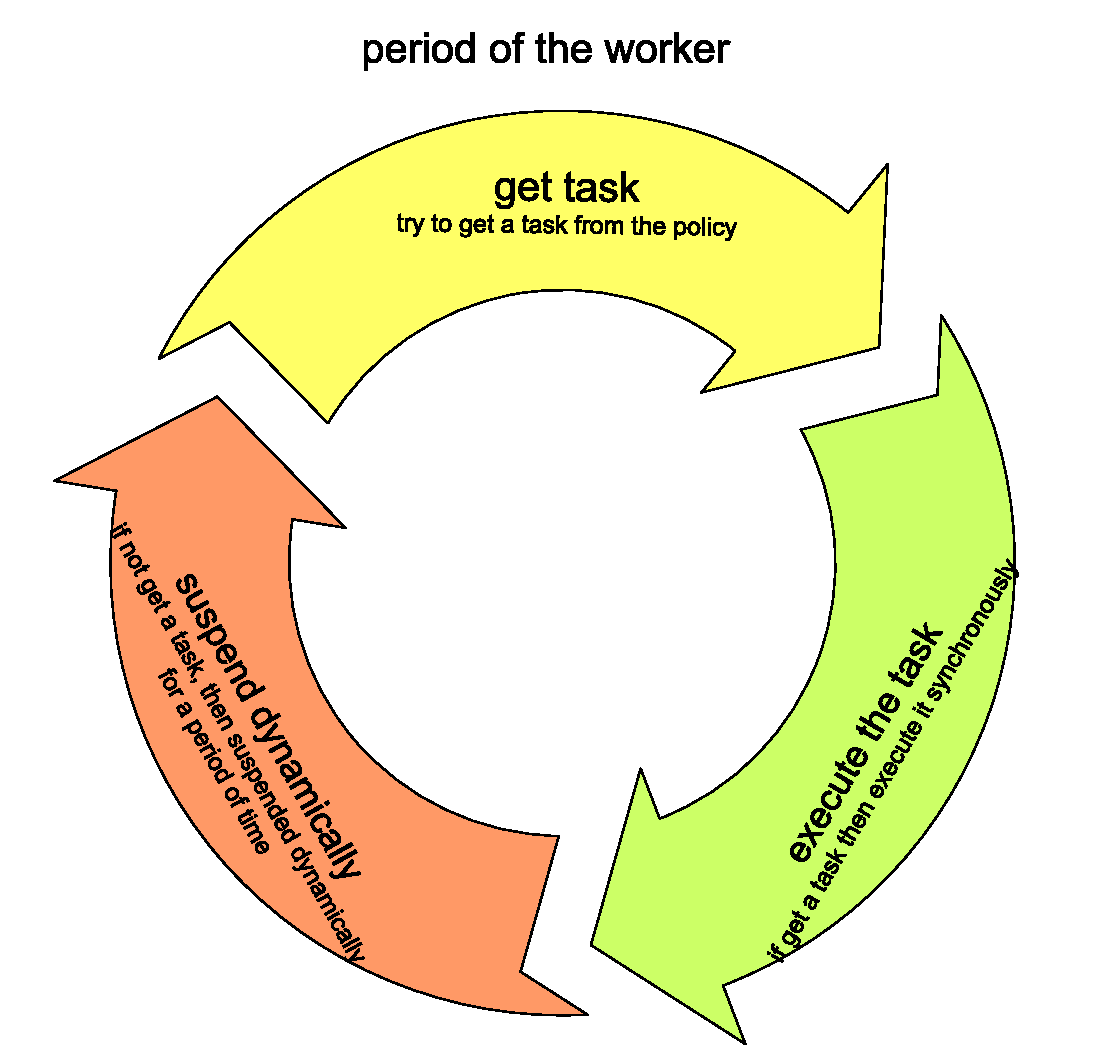
\includegraphics[width=0.7\textwidth]{images/period_of_worker.pdf}
    \caption{Period of the Worker}
    \label{fig:period_of_worker}
\end{figure}
\FloatBarrier

It is evident that each worker, from creation to termination,
exists within a loop comprising three possible stages:
\begin{enumerate}
    \item Invoking the getWork function from Policy to acquire tasks;
    \item If tasks are acquired, they are executed;
    \item If no tasks are acquired, the worker sleeps for a duration.
          This duration increases with each unsuccessful task retrieval attempt and resets upon a successful retrieval.
\end{enumerate}

Among these stages, the first is invariably experienced in every cycle,
while the second and third stages are mutually exclusive, with only one transpiring per cycle.

To analyze the actual load of a worker, focus must be placed on the second stage,
since it represents the phase where the worker genuinely processes tasks.
The time consumed during this phase represents the effective load duration,
while the time consumed in other phases can be categorized as idle time,
given that no tasks are executed, rendering it ineffective load time.

Considering that the original cycle might not necessarily undergo the second phase,
to prevent the update of redundant data,
this paper redefines the lifecycle judgment of the worker.
The conclusion of one task execution marks the commencement of a new cycle,
while the initiation of a task signals the end of a cycle.
This ensures that each cycle invariably undergoes the second phase,
which is the task execution phase.

Building upon this theoretical foundation,
we have designed a comprehensive data collection scheme as depicted in \cref{fig:worker_collect_calculate}.

\begin{figure}[h]
    \centering
    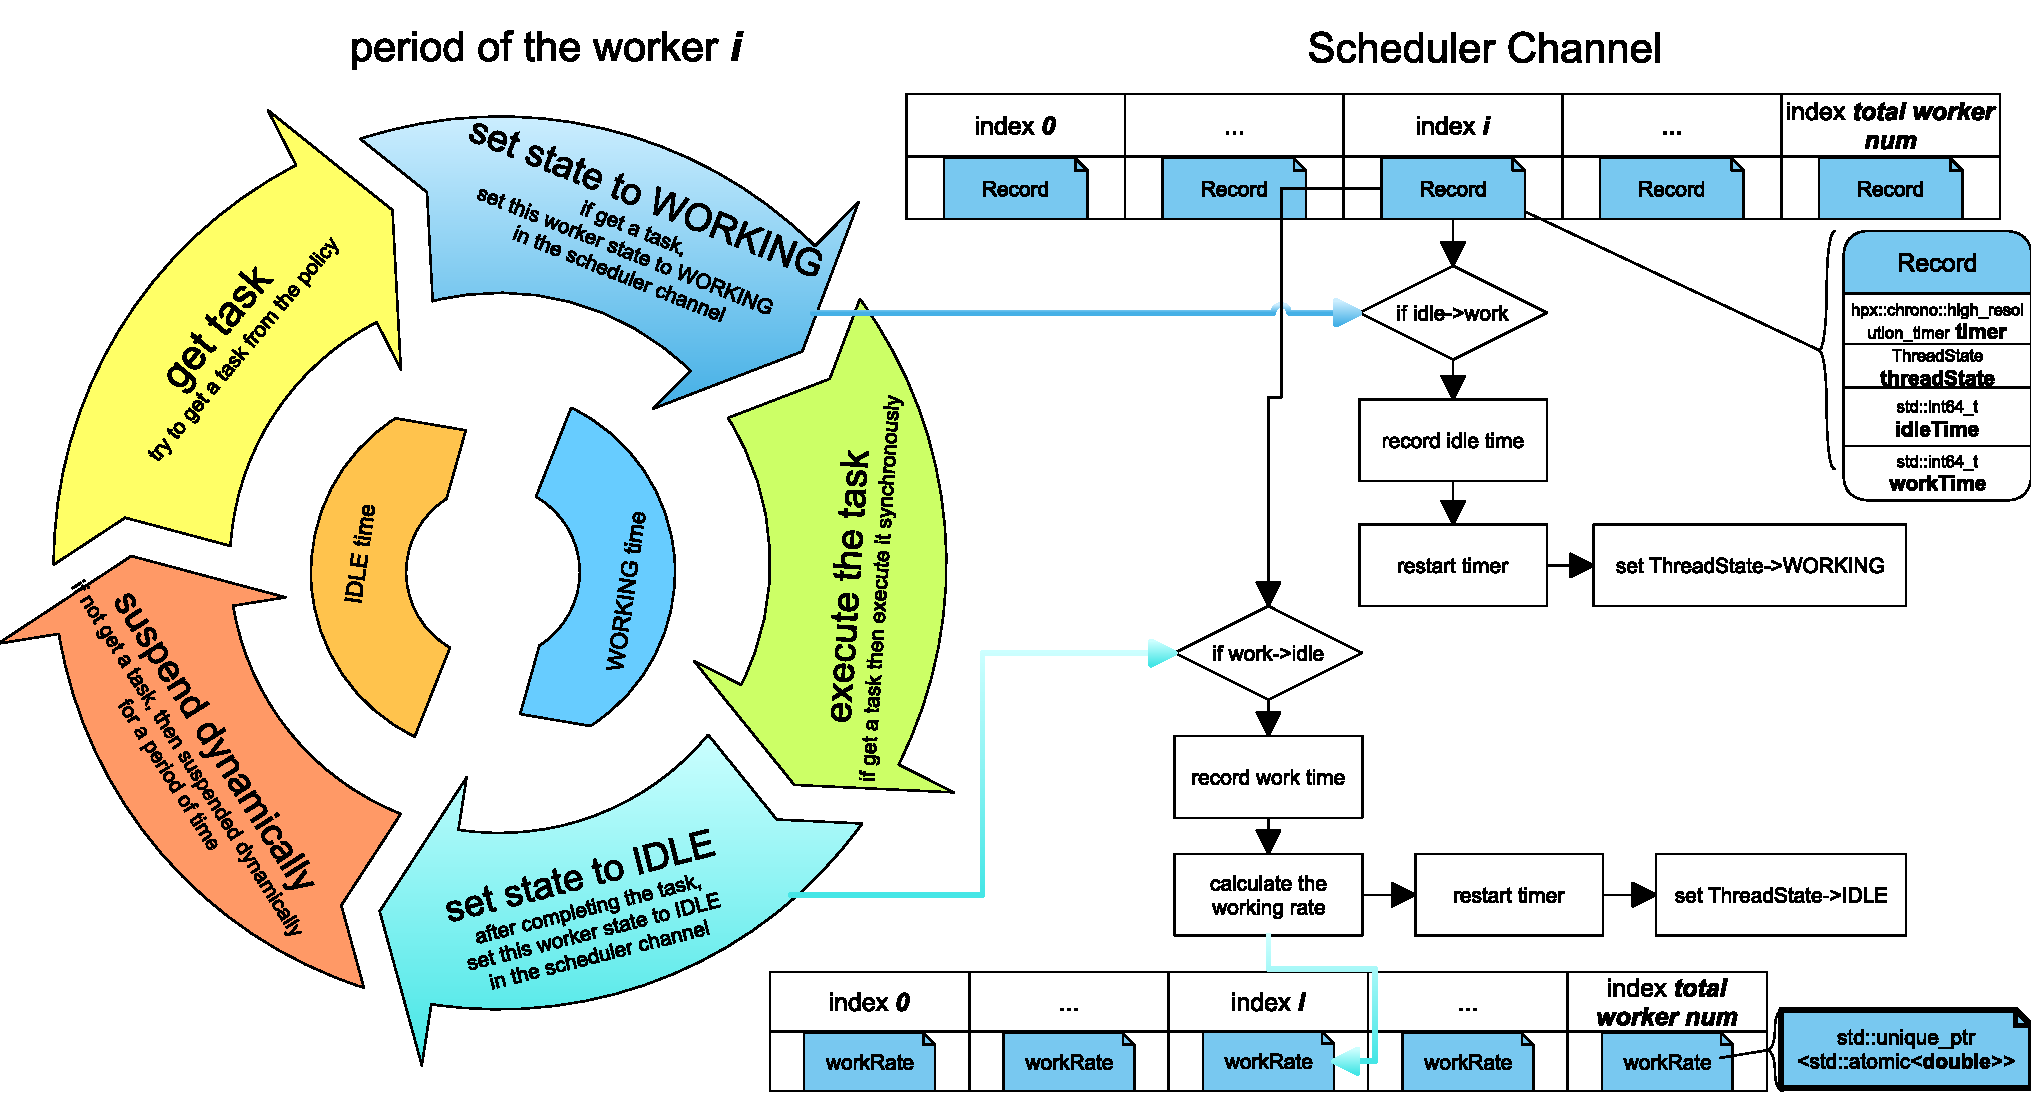
\includegraphics[width=1.0\textwidth]{images/worker_collect_calculate.pdf}
    \caption{Collect Worker State to Calculate the Workload}
    \label{fig:worker_collect_calculate}
\end{figure}
\FloatBarrier

By inserting probing code at the beginning and end positions of task execution
(which, upon execution, momentarily halts the current process and proceeds with probe-related operations),
a worker can update its status to the Scheduler Channel module (a channel dedicated to status transmission)
before and after executing a task.
In this manner, the worker can compute and update its load data in real-time,
supplying the Performance Monitor with the requisite data for further calculations.

The Scheduler Channel employs a specific data structure for data aggregation.
To circumvent the overheads associated with lock usage,
it adopts a lock-free design strategy as discussed in \cref{survey_lock}.
This design aims to mitigate contention among workers when collecting load data.

This data structure principally consists of two arrays, each with a length equivalent to the number of local workers:
\begin{enumerate}
    \item Record Array: This array stores distinct Record data structures. Each Record encompasses:
          \begin{itemize}
              \item A timer, denoted as 'timer'
              \item The current status, termed 'threadState'
              \item Idle time for the current cycle, labeled 'idleTime'
              \item Working time for the current cycle, named 'workTime'
          \end{itemize}
          Such a design allows workers to log their durations under various states.
          As each worker corresponds to an individual record,
          it avoids the need for locks, thereby enhancing performance.
    \item workRate Array: This array retains the worker load rate data, computed through a specific algorithm.
          Each 'workRate' is an atomic double type wrapped by 'unique\_ptr'.
          Although both the worker and Monitor might access this data concurrently,
          the fundamental datatype nature of 'workRate' ensures data integrity in a lock-free environment using the atomic type.
\end{enumerate}

The load data collection here primarily consists of two workflows:
\begin{itemize}
    \item During the "set state to WORKING" phase,
          the worker primarily updates its idle time for this cycle in the channel and switches its state to WORKING.
    \item During the "set state to IDLE" phase,
          the worker primarily updates its working time for this cycle in the channel.
          Based on the idle and working time, along with historical workRate data,
          it calculates the current workRate and switches its state to IDLE.
\end{itemize}

During the "set state to IDLE" phase, the algorithm to compute the latest workRate is presented in \cref{eq:workrate}:

\begin{align}
    \text{workRate} & = \left( \ln\left( 2.72 + \frac{\text{workTime}}{\text{workTime} + \text{idleTime}} \right) \right. \notag   \\
                    & \qquad \times \left. \ln\left( 2.72 + (\text{workTime} + \text{idleTime}) \right) \times 0.65 \right) \notag \\
                    & \qquad + \text{workRate} \times 0.35 \label{eq:workrate}
\end{align}

The purpose of the formula is to gauge whether the current worker is busy and whether its computing speed is relatively slow. It comprises three main components:
\begin{enumerate}
    \item $\ln\left( 2.72 + \frac{\text{workTime}}{\text{workTime} + \text{idleTime}} \right)$:
          Within each cycle, if the duration of the WORKING state relative to the IDLE state is greater,
          it indicates a substantial or complex task load, necessitating more time for task execution.
          Conversely, a prolonged task starvation time signifies significant time wastage on unproductive load,
          such as speculative task stealing.
          Given that time data is measured in microseconds and exhibits substantial variability,
          a logarithmic function is employed to temper data sensitivity,
          and the term $(2.72+...)$ ensures a positive outcome.

    \item $\ln\left( 2.72 + (\text{workTime} + \text{idleTime}) \right)$:
          The prior ratio doesn't adequately reflect the current worker's execution speed.
          There might be cases where the task load is minimal,
          but due to a slow execution speed, the actual load remains significant.
          By calculating the total duration for the current cycle and multiplying it by the previously computed ratio,
          one can obtain a practical load scenario for the cycle.
          The logarithmic function, given its microsecond-level granularity, is also employed here to reduce data sensitivity.

    \item $(... \times 0.65 +\text{workRate} \times 0.35)$:
          Refreshing data might occur after intervals.
          Retaining historical load data as a reference, to prevent misjudgment due to short-term fluctuations, is essential.
          Since the current load rate data structure is optimized for memory efficiency and doesn't maintain structures like arrays for historical data,
          an exponential smoothing technique, as referenced in \cite{GARDNER2006637},
          is adopted to balance current and historical workRate data.
          The coefficients 0.65 and 0.35 were determined through extensive cluster environment testing
          to make the data more smooth and informative.
\end{enumerate}

In the end, the workRate data computed for each worker is aggregated and divided by the number of workers to derive the average load data.
This processed data is a lightweight double type, which is then passed to the Performance Monitor.
The monitor submits this local workRate data to the local distributed component, facilitating rapid queries by other nodes.

\subsection{Collection of Residual Task Volume and Communication Latency}\label{collect_tesks_delay}

Performance data also requires the collection of residual task volume and acquisition time for each node,
as illustrated in \cref{fig:tasks_detection}.

\begin{figure}[h]
    \centering
    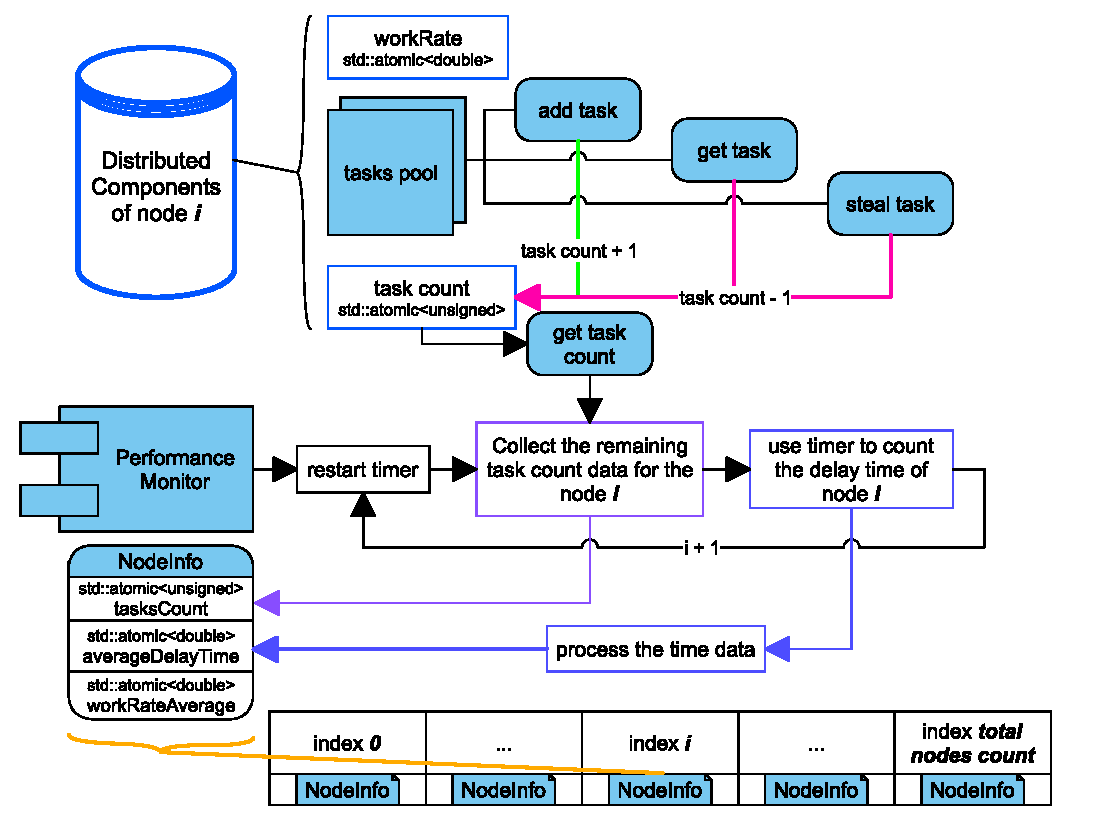
\includegraphics[width=0.98\textwidth]{images/tasks_detection.pdf}
    \caption{collect tasks count and delay time}
    \label{fig:tasks_detection}
\end{figure}
\FloatBarrier

The distributed component in HPX comprises a task pool and the number of residual tasks.
The count of the residual tasks, introduced in a later phase for the needs of this framework,
employs a lightweight atomic type to ensure data integrity.
Originally, the task pool had three distributed operations to modify it:
adding tasks, retrieving tasks, and stealing tasks.
To maintain the accuracy of the residual task count,
updates are made during these operations as depicted in \cref{fig:tasks_detection}.
Within each node's Performance Monitor,
a routine will traverse and invoke the get\_task\_count interface of each node's distributed component to obtain the residual task count.

To quantify the communication delay between the local node and other nodes,
which represents the time required to retrieve data between distributed components,
the delay in obtaining the residual task count from each node is measured.
This process, while fetching distributed component data,
also captures communication delay without incurring additional IO overhead.

It's worth noting that the communication delay also subtly reflects the busyness of the node's thread pool.
Since the task count uses atomic types,
an active thread pool may occasionally block other modification operations,
resulting in increased time to retrieve the task count.

Given that the obtained communication delay is a temporal datum,
which could exhibit significant values and fluctuations, it requires further processing before storage.
The processing formula is:

\begin{align}
    \text{averageDelayTime}_i & = \ln\left(2.72 + \text{delayTime} \times \text{worker\_count}\right) \times 0.65 \notag               \\
                              & + \text{nodeInfoVector}[i]\texttt{->}\text{averageDelayTime} \times 0.35   \label{eq:averageDelayTime}
\end{align}

Here, $i$ represents the identifier for each node.
As node identifiers remain consistent within the HPX framework,
they can serve as array indices for easy node location.
$\text{delayTime}$ denotes the communication delay, and $\text{worker\_count}$ is the count of workers on the node.
Firstly, the formula multiplies the delay time by the local worker count to reflect the node's overall communication overhead.
Similar to \cref{eq:workrate}, logarithmic functions and exponential smoothing are applied to reduce data sensitivity,
retaining some impact from historical data,
making the results smoother and more informative.

After processing, the data is stored.
The storage data structure also adopts a lock-free design,
as shown in \cref{fig:tasks_detection}.
It's an array with a length equal to the total number of nodes,
with index numbers corresponding to node identifiers.
Stored within the array is a structure called NodeInfo,
which contains atomic-type node load rates, residual task counts, and average communication delays for the corresponding node.

\section{Optimal Steal Target Calculation and Caching}

Upon acquiring performance data such as node load status, residual task volume on each node,
and communication latency through the performance collection mechanism in the Performance Monitor,
the optimal steal target node is calculated using these data.
The node's ID is then cached for subsequent retrieval by the Performance Policy.
The overall process is illustrated in \cref{fig:refresh_target}.

\begin{figure}[h]
    \centering
    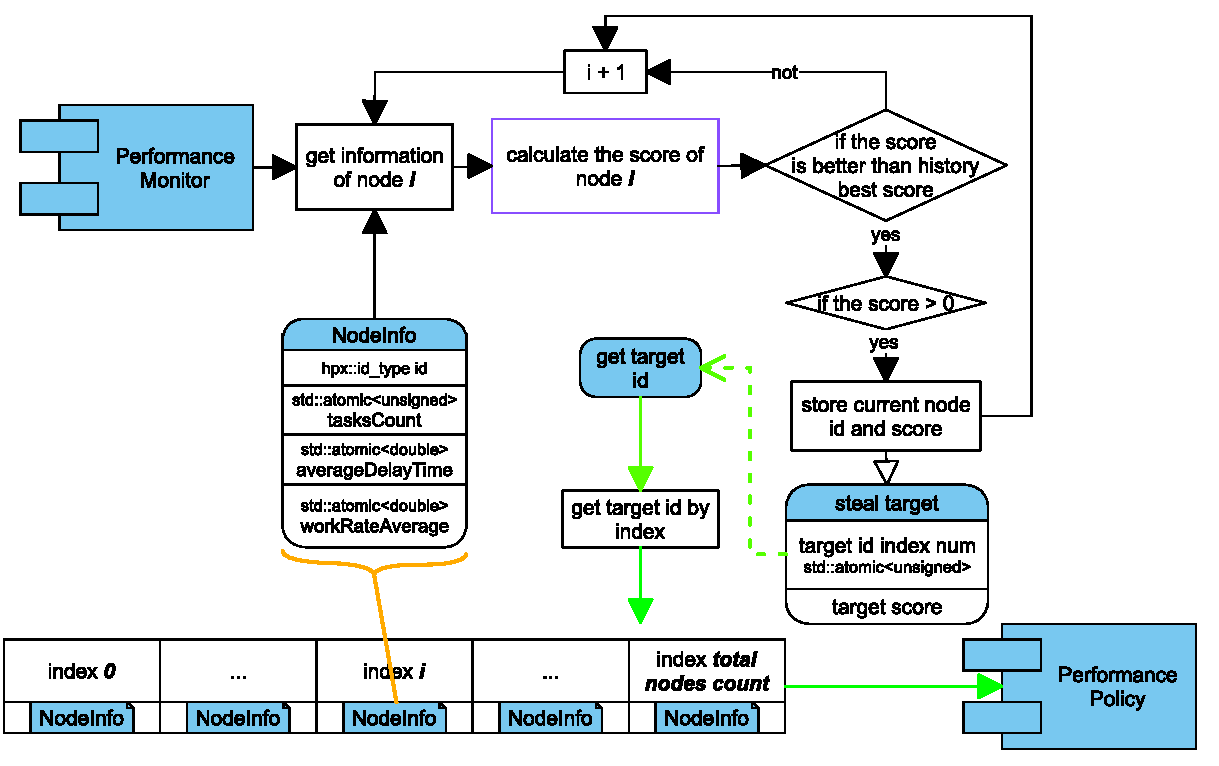
\includegraphics[width=1\textwidth]{images/refresh_target.pdf}
    \caption{refresh the optimal steal target}
    \label{fig:refresh_target}
\end{figure}
\FloatBarrier

The array data structure has been introduced earlier in \cref{collect_tesks_delay}.

The procedure starts by iterating through the NodeInfo data structure of each node to calculate the steal-worthiness score.
A higher score indicates a higher worthiness for task stealing.
Its formula is:

\begin{align}
    \text{score}_i & = \max\left(\text{nodeInfoVector}[i]\texttt{->}\text{workRateAverage}, 0.0001 \right) \notag \\
                   & \quad\times \text{nodeInfoVector}[i]\texttt{->}\text{tasksCount} \notag                      \\
                   & \quad - \text{nodeInfoVector}[i]\texttt{->}\text{averageDelayTime} \label{eq:score}
\end{align}

The core idea behind this formula is to reduce the task volume of the most heavily-loaded nodes while also minimizing the time wasted in task stealing.
The formula can be broken down into:

\begin{enumerate}
    \item Using $\max\left(\text{nodeInfoVector}[i]\texttt{->}\text{workRateAverage}, 0.0001 \right)$ to avoid interference from negligibly small data in computations.
    \item Multiplying the node's load rate by its residual task count, $\times \text{nodeInfoVector}[i]\texttt{->}\text{tasksCount}$, provides an estimate of the node's total load.
    \item Subtracting the communication latency, $- \text{nodeInfoVector}[i]\texttt{->}\text{averageDelayTime}$, ensures minimal time wastage during task stealing.
\end{enumerate}

A larger result suggests that the node is more deserving of task stealing because it has a larger workload and will require more time to process residual tasks.
Moreover, its communication latency is smaller, meaning less time is wasted during the task-stealing process.

After iterating through all nodes, an optimal node target index is typically identified and cached.
When the Performance Policy needs to retrieve the optimal steal target's $id\_type$, it can do so through a provided query interface.
This design is partly because HPX's $id\_type$ is not a basic data type and cannot be atomized.
However, the corresponding array index number can be atomized.
To maintain a lock-free design and avoid resource wastage due to prolonged blocking, the refresh phase only modifies the stored index number.
During the query phase, the $id\_type$ of the optimal target node is retrieved using the index number.
This ensures that all $id\_type$ values are only read, not modified, guaranteeing data safety in a lock-free environment.

The worthiness of the selected optimal steal target is judged based on:
\begin{itemize}
    \item Whether there are any residual tasks left to steal from the target.
    \item Whether the cost of stealing outweighs the benefits, i.e., if the time spent on stealing tasks exceeds the time saved by assisting the target node in completing tasks.
\end{itemize}
Under such circumstances, the score is often less than or equal to zero.
Hence, an additional condition is set to not cache the optimal steal target if the score is less than or equal to zero.
In this case, under the Performance Policy, the worker will attempt to retrieve the optimal steal target again.
If unsuccessful, it will enter a brief sleep mode to avoid wasting computational resources with frequent attempts.

\section{Refresh Data and Provide Tasks Mechanism}

After establishing a mechanism that spans from data collection to calculating and caching the optimal steal target,
the next challenge to address is determining the frequency of data refresh.
Although the overhead of each data refresh is relatively small,
YewPar's workers are designed to fully utilize local computational resources.
Therefore, when workers are busy, too frequent refreshes can interrupt their operations,
potentially impacting YewPar's performance.
On the other hand, infrequent refreshes might reduce data reliability due to outdated information.
This can result in providing inaccurate data to other nodes or relying on stale cached data from other nodes.
In the worst-case scenario, this might lead to stealing tasks from already starved nodes, exacerbating imbalances.

To address this issue, this paper proposes a bidirectional dynamic refresh mechanism.
This mechanism consists of two refresh methods: an automatic dynamic refresh method and an auxiliary refresh method facilitated by the Performance Policy.
The general workflow is depicted in \cref{fig:refresh_provide}.

\begin{figure}[h]
    \centering
    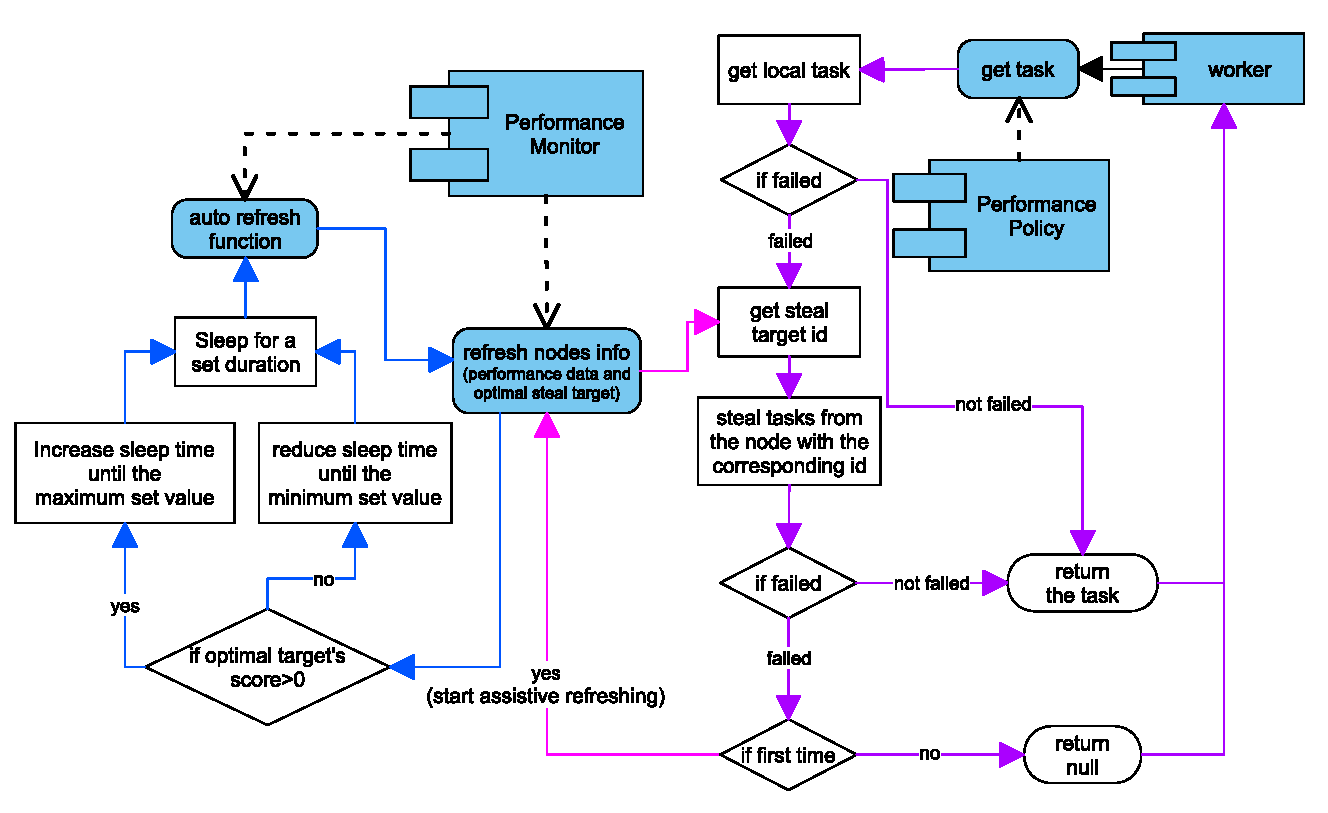
\includegraphics[width=0.98\textwidth]{images/refresh.pdf}
    \caption{refresh data and provide tasks mechanism}
    \label{fig:refresh_provide}
\end{figure}
\FloatBarrier

On the left side of the diagram, an automatic dynamic refresh task is deployed within the Performance Monitor.
At its core, this task is iterative, adjusting the timing of the next refresh based on the results of the previous one.
If the refresh results are suboptimal, it's likely that some workers are still starved.
In such cases, the subsequent refresh time will be significantly shortened.
Conversely, if results align with expectations, indicating that most workers are likely to successfully acquire tasks,
the time until the next refresh will be gradually extended to minimize unnecessary interruptions.
Currently, the optimality of the refresh is primarily judged by the score.
If the score is less than or equal to zero, it is considered suboptimal.
According to \cref{eq:score}, this is likely due to a scarcity of tasks in the pool or excessive time taken to obtain tasks.
Under such conditions, the cost of task stealing might outweigh the benefits.

It's worth noting that while dynamically adjusting the refresh time yields noticeable benefits in practice,
upper and lower limits should still be imposed.
A lack of an upper limit might lead to using stale data, resulting in the caching of suboptimal steal targets.
Without a lower limit, frequent refreshes could potentially disrupt the performance of workers with ongoing tasks or impact system-level scheduling.
Through extensive experimentation, a range has been identified that minimizes impact on system performance while ensuring relative data timeliness.
Furthermore, incorporating algorithms like exponential smoothing retains the influence of historical data,
ensuring that even slightly delayed data accurately reflects the overall status of nodes.

However, there's still room for improvement and optimization in the aforementioned design.
Thus, as shown on the right side of \cref{fig:refresh_provide}, an auxiliary refresh mechanism facilitated by the Performance Policy has been introduced.
The essence of the Performance Policy is a task retrieval strategy.
It prioritizes acquiring local tasks since doing so allows workers to quickly obtain and execute tasks, minimizing resource wastage.
If local tasks are unavailable, the policy will first query the Performance Monitor's cached optimal steal target id.
While this typically results in a successful task steal, there are scenarios where very few tasks remain across all nodes,
leading to occasional unsuccessful steals.
If the automatic refresh mechanism is dormant and unable to promptly adjust the refresh rate,
the Performance Policy, when invoked by a worker, assumes the role of an auxiliary refresher.
After the data refresh is complete, another attempt is made to steal tasks based on the new target.
If this too fails, it's highly probable that very few tasks are available across nodes.
To conserve communication resources, the worker will then enter a sleep cycle to reduce resource consumption.

In practice, the combined effect of both mechanisms has been observed to significantly enhance system performance.


%%%%%%%%%%%%%%%%%%%%%%%%%%%%%%%%%%%%%%%%%%%%%%%%%%%%%%%%%%%%%%%%%%%

\chapter{Evaluation}

\section{Search Applications}

We evaluated the performance of the improved workstealing strategy on representative search applications and samples for the two types of searches initially present in YewPar, as shown below:

\begin{itemize}
    \item Enumeration:
          Unbalanced Tree Search (UTS) dynamically constructs synthetic irregular tree workloads based on a given branching factor, depth, and random seed\cite{olivier2006uts}.
          Number Semigroups (NS) calculates how many number semigroups exist for a specific genus\cite{fromentin2016exploring}.
          A number semigroup S is a residual set of natural numbers that includes 0 and is closed under addition;
          the genus of S is the size of its complement.
    \item Optimisation:
          Maximum Clique (MaxClique) identifies the largest clique in a given graph, i.e., the largest set of pairwise adjacent vertices.
          The 0/1 Knapsack problem determines the best combination of items, each with a profit and weight, to place in a container,
          ensuring maximum profit within a given weight constraint.
          The Traveling Salesman Problem (TSP) finds the shortest possible round trip through N cities.
\end{itemize}

To control variables, the evaluation utilized the Maxclique-16 and NS-hivert applications that come with the hpx1.8 branch of YewPar without any modifications.
However, at runtime, we employed both the modified Performance-Driven Workstealing Policy and the original hpx1.8 branch's DepthPool Policy for comparison.
The baseline implementations of MaxClique\cite{mccreesh2013multithreading} and NS\cite{fromentin2016exploring} employed publicly advanced algorithms.
These sequential C++ implementations were provided by domain experts.
A comprehensive description of the applications and instances can be found in \cite{archibald2018}.

For the Maxclique-16 application, the larger dataset brock800\_2.clq was used to prolong runtime and minimize comparative errors.
We adopted the Depth-Bounded skeleton, which is more suitable for the Maxclique-16 application and can utilize the Performance-Driven Workstealing Policy.
We set the parameter \(d = 2\) (spawn-depth: Depth in the tree to spawn at) as, in practice, we found that when \(d\) is set to 2, it offers superior performance and stability compared to other parameters.

For NS-hivert, the Budget skeleton was employed, being more suitable for the NS-hivert application and compatible with the Performance-Driven Workstealing Policy.
Parameters were set as \(b = 10^6\) (backtrack-budget: Number of backtracks before spawning work) and \(g = 47\) (genus: Depth in the tree to count until) to ensure accurate results while increasing the workload to prolong runtime and thus reduce statistical errors.

\section{Experimental Setup}

We conducted measurements on the program's execution across as many as 20 machines.
Each machine was equipped with a dual 8-core Intel Xeon E5-2640v2 2GHz CPU (without hyper-threading),
64GB RAM, and was running the Ubuntu 22.04.2 LTS operating system.
Before testing, each machine maintained a load within 1\%.
Similar to the original hpx1.8 branch of YewPar, we reserved one core for task management for HPX (version 1.8),
thus utilizing 15 working threads out of the 16 cores available.

It's essential to note that, due to the non-determinism caused by pruning, the search for alternative effective solutions, and the high randomness of the original YewPar's workstealing scheme,
performance analysis in parallel search is highly challenging.
This can potentially lead to performance anomalies, as referenced in \cref{sec:performance_anomalies},
manifesting as super-linear speed-ups/slowdowns.
To control these factors,
we ran each program multiple times under various node quantities (set to 10 times)
and reported the aggregated statistical data.

The code used for the experiments,
along with installation instructions and detailed experimental specifics (including the commands used and data obtained),
can be found in the \cref{appendix:link}.

\section{Isolated Performance Evaluation of Different Policies}

To precisely assess the performance difference between the YewPar based on the Performance-Driven Workstealing Policy and the original version under an idle environment,
we conducted individual test evaluations on two applications when all nodes were in an idle state.
To minimize test errors,
we opted to alternate between the modified and original versions of the application.
That is, after running the program based on the modified Policy framework,
we immediately ran the program based on the original Policy,
followed by another run of the program based on the modified Policy framework.
This cycle was repeated until all test rounds were completed.
During these tests, the running program had exclusive access to all computational resources.

\subsection{Isolated Performance Evaluation of Maxclique}

The results for the run time of the Maxclique program based on the Depth-Bounded skeleton, averaged over ten runs, are presented in \cref{fig:time_comparison_max_solo}.
The results are divided into two sections: run-time evaluation and a comparison of the performance improvement of the Performance-Driven Workstealing Policy over the original DepthPool Workstealing Policy.

The formula for calculating the speed improvement is given by
\begin{equation}
    \text{Speedup Percentage} = \left( \frac{T_{\text{DepthPool}} - T_{\text{Performance-Driven}}}{T_{\text{Performance-Driven}}} \right) \times 100\%
\end{equation}
where \( T_{\text{DepthPool}} \) is the run-time of the application based on the original YewPar's DepthPool Workstealing Policy,
and \( T_{\text{Performance-Driven}} \) is the run-time of the application based on the Performance-Driven Workstealing Policy.

\begin{figure}[h]
    \centering % Center the image
    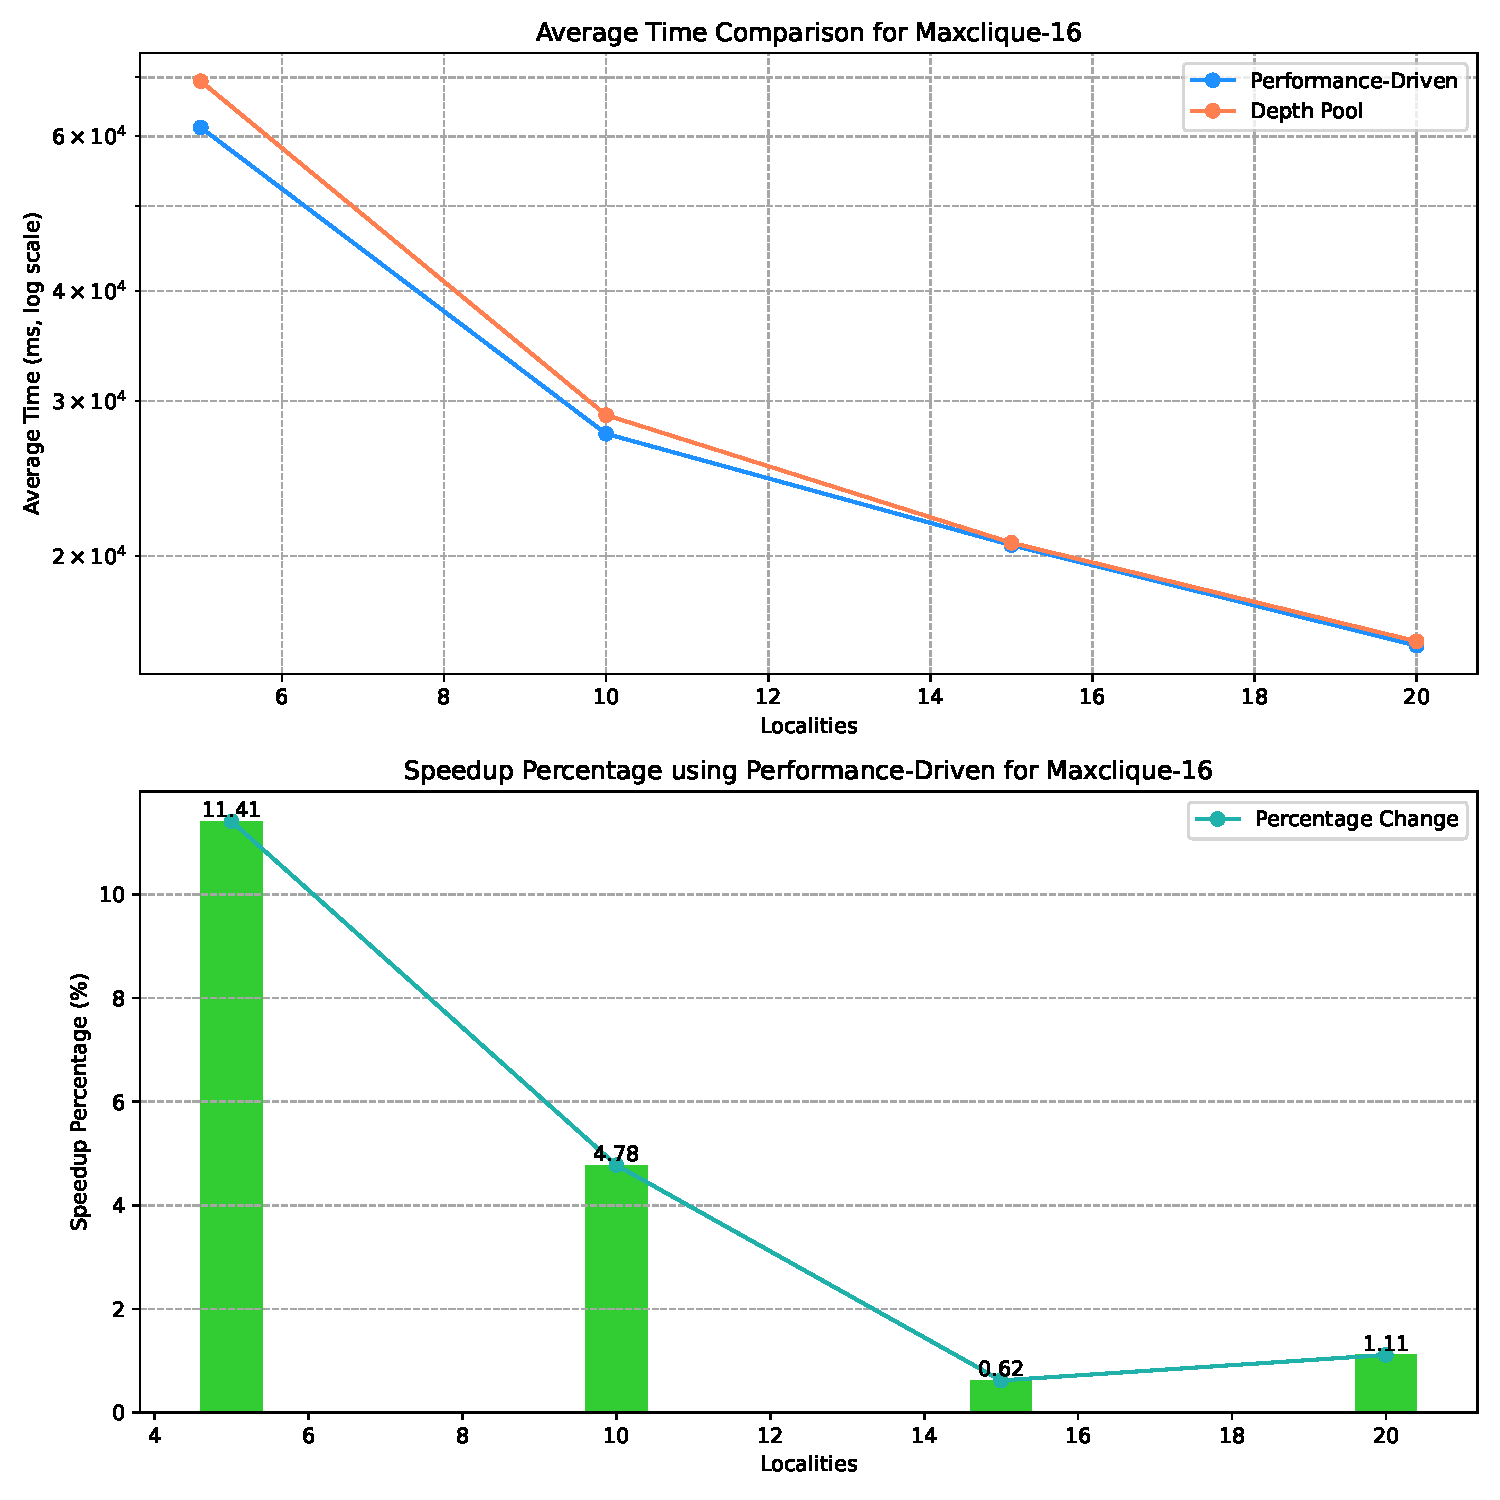
\includegraphics[width=0.9\textwidth]{images/time_comparison_max_solo.pdf} % Insert the image, setting the width to 80% of the text width
    \caption{isolated time comparison for Maxclique-16} % Provide a caption for the image
    \label{fig:time_comparison_max_solo} % Provide a label for the image for referencing elsewhere in the document
\end{figure}
\FloatBarrier

From the graph, it is evident that, when run in isolation and across varying node counts,
the YewPar based on the Performance-Driven Workstealing Policy consistently outperforms the YewPar based on the original DepthPool Workstealing Policy,
completing all tasks in a shorter time.

However, from the graph, it's evident that between the range of 5 to 15 nodes,
the speed improvement diminishes from its peak of 11.41\% at 5 nodes to a low of 0.62\% at 15 nodes,
only to rise again to 1.11\% at 20 nodes.
Theoretically, as the number of nodes increases,
the potential for optimizing the Workstealing target should also grow,
resulting in a more pronounced speed improvement.
To understand this anomaly, we undertook an analysis:
\begin{itemize}
    \item An analysis of the Performance-Driven Workstealing Policy revealed minor factors such as increased overhead due to data collection and computation resulting from additional nodes.
          However, in theory, this overhead should be negligible when compared to the benefits of optimized workstealing targets.
    \item A deeper investigation into the application's implementation and specific test data suggested the primary issue likely stemmed from performance anomalies referenced in \cref{sec:performance_anomalies}.
          The Maxclique program based on the Depth-Bounded skeleton exhibited a higher probability of super-linear deceleration compared to other applications.
          To validate this hypothesis, beyond analyzing the YewPar code,
          we also studied the runtime fluctuations of the Maxclique program based on the Depth-Bounded skeleton.
          Using the data from a 10-node test as an example, the fluctuations are depicted in \cref{fig:maxclique_16_fluctuations}.
          \begin{figure}[h]
              \centering
              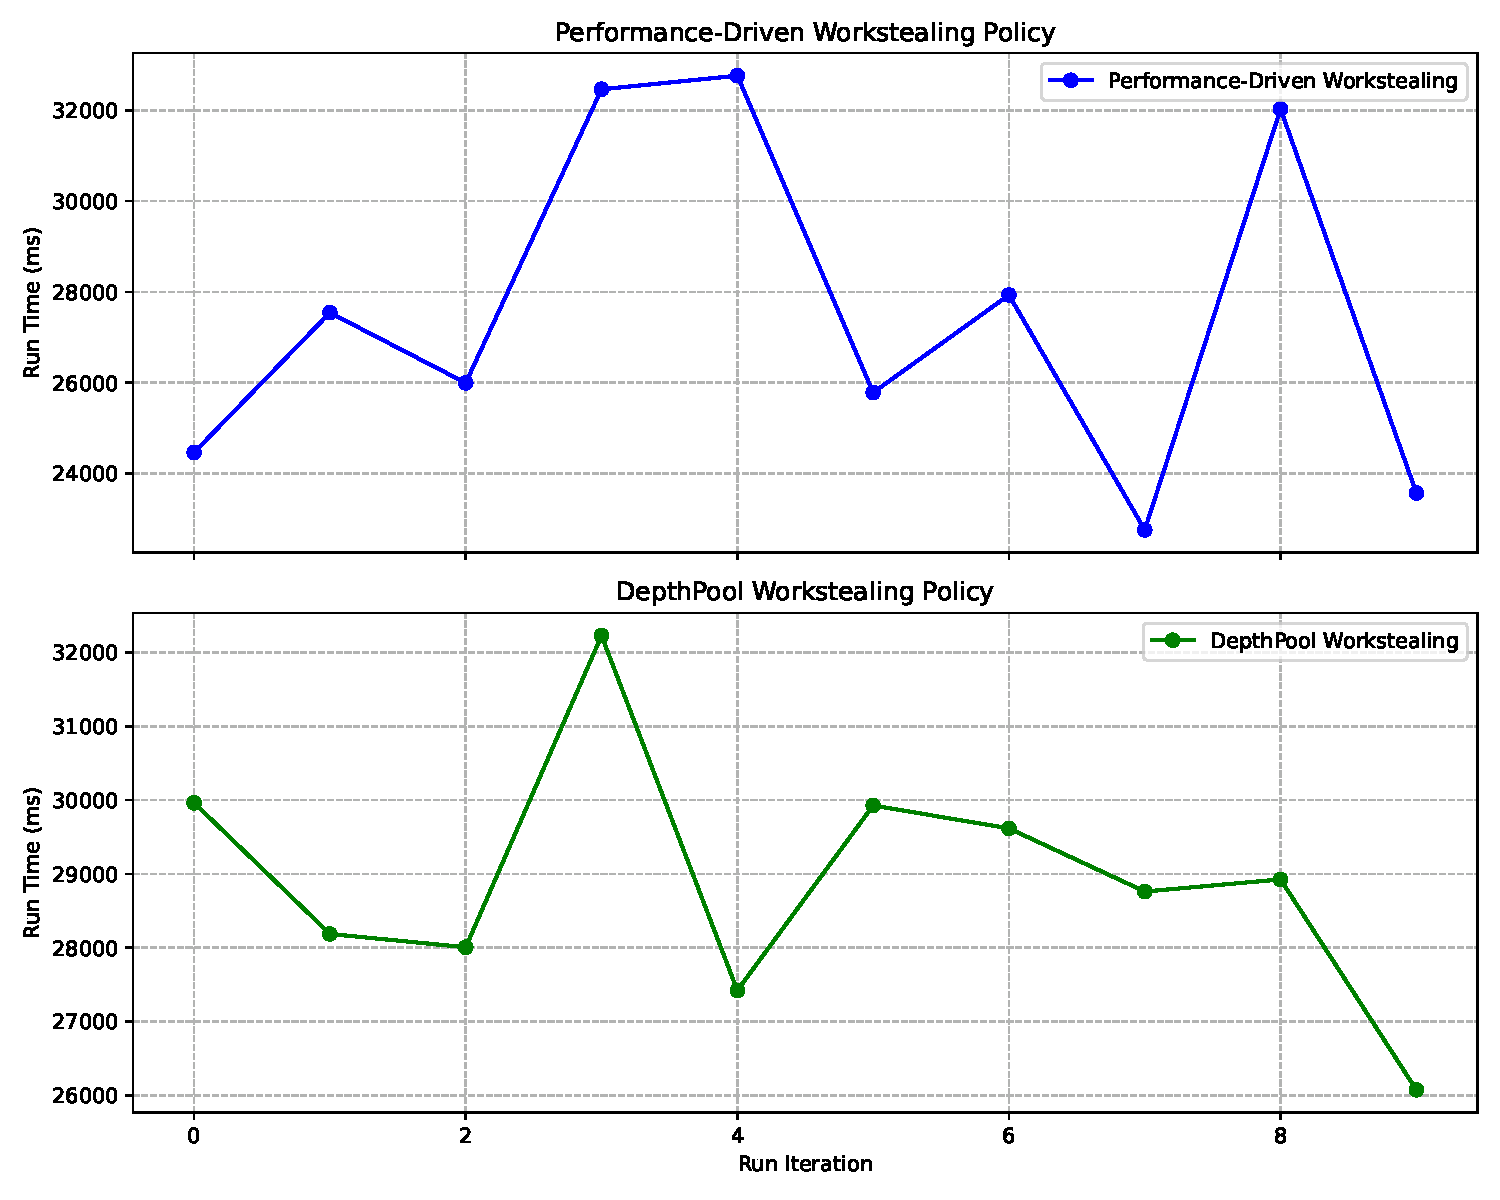
\includegraphics[width=0.8\textwidth]{images/maxclique_16_fluctuations.pdf}
              \caption{Runtime fluctuations for Maxclique-16 application based on two different policies using 10 localities.}
              \label{fig:maxclique_16_fluctuations}
          \end{figure}
          \FloatBarrier
          When evaluating the runtime variability of the Maxclique-16 application,
          we calculated the percentage difference between the maximum and minimum values using the formula:
          \begin{equation}
              \text{Variability Percentage} = \left( \frac{\text{Max Value} - \text{Min Value}}{\text{Min Value}} \right) \times 100\%
              \label{eq:variability_percentage}
          \end{equation}
          \FloatBarrier
          The Maxclique-16 application based on the Performance-Driven Workstealing Policy had a maximum variability percentage of 43.98\%.
          In contrast, the application based on the DepthPool Workstealing Policy had a maximum variability percentage of 23.61\%.
          It's clear that the Maxclique program's runtime based on the Depth-Bounded skeleton already exhibited significant variability,
          but the variability of the Maxclique program based on the Performance-Driven Workstealing Policy was nearly double.
          Considering the content of performance anomalies in \cref{sec:performance_anomalies},
          it's evident that the Maxclique program might disrupt the search heuristic more with the addition of computational resources,
          leading to an increase in extraneous tasks.

          Although the frequent changes in the Workstealing target might result in the generation of extra tasks,
          it's worth noting in \cref{fig:time_comparison_max_solo} that between 15 and 20 nodes,
          there's a relative speed increase.
          This can likely be attributed to the benefits of optimized Workstealing targets progressively outweighing the detriments caused by the additional tasks.
\end{itemize}

\subsection{Isolated Performance Evaluation of NS-hivert}

For the NS-hivert program based on the Budget skeleton, the results after averaging the runtimes from ten iterations for each test set are depicted in \cref{fig:time_comparison_ns_solo}.
The evaluation encompasses both runtime assessment and the speed improvement evaluation comparing the Performance-Driven Workstealing Policy to the original DepthPool Workstealing Policy.

\begin{figure}[h]
    \centering
    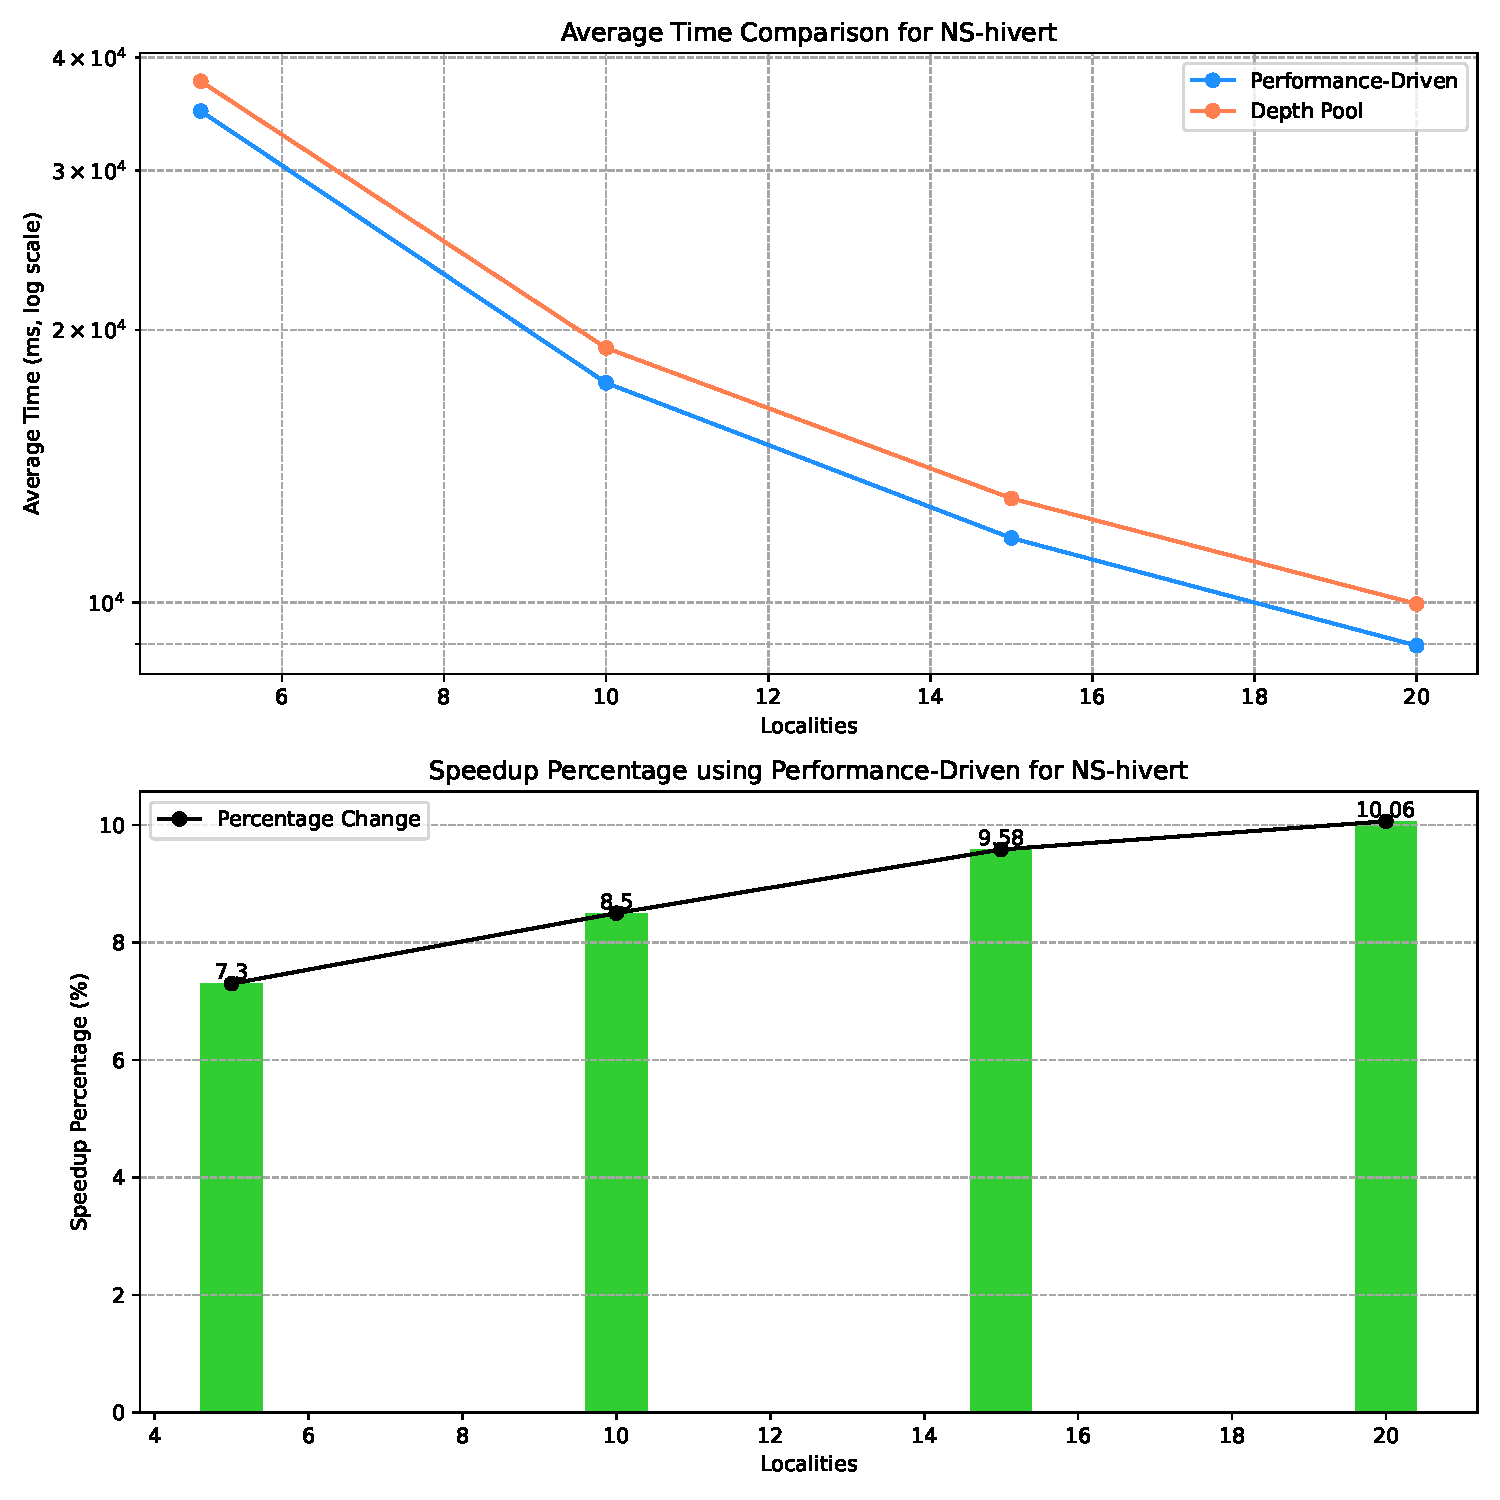
\includegraphics[width=0.9\textwidth]{images/time_comparison_ns_solo.pdf}
    \caption{isolated time comparison for NS-hivert}
    \label{fig:time_comparison_ns_solo}
\end{figure}
\FloatBarrier

From the graph, it's evident that when run in isolation, the NS-hivert program based on the Performance-Driven Workstealing Policy exhibits superior performance across different node counts, completing all tasks in a shorter duration.
The speed improvement escalates with the increase in node count.
At 20 nodes, there's an average speed increment of 10.06\%.
Considering this enhancement is solely achieved by adjusting the Workstealing Policy without any modifications to other parts of YewPar and despite the adverse impacts of performance anomalies referenced in \cref{sec:performance_anomalies}, this result is commendable.

Contrasting with the Maxclique program, the speed improvements attributed to the Performance-Driven Workstealing Policy are more pronounced here as node counts increase.
This is primarily because the NS-hivert program experiences fewer adverse effects from performance anomalies as discussed in \cref{sec:performance_anomalies}.
We also analyzed the runtime variability of the NS-hivert program, as shown in \cref{fig:NS_hivert_fluctuations}.

\begin{figure}[h]
    \centering
    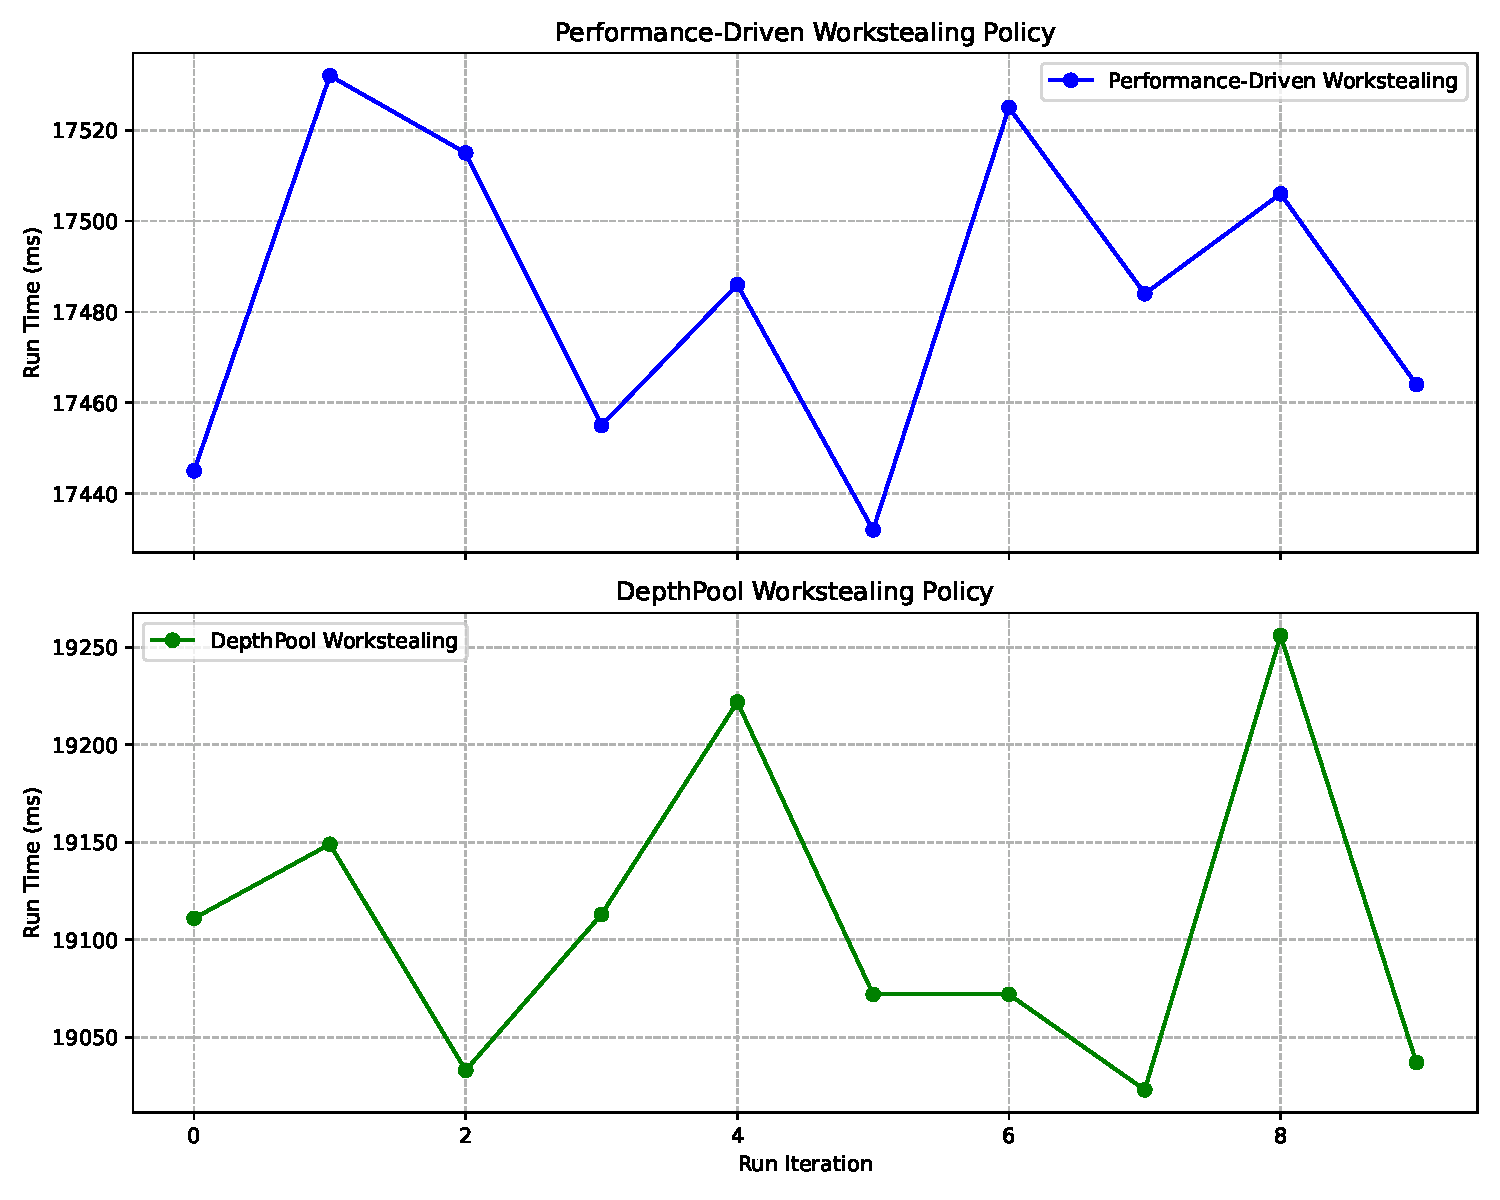
\includegraphics[width=0.8\textwidth]{images/NS_hivert_fluctuations.pdf}
    \caption{Runtime fluctuations for NS-hivert application based on two different policies using 10 localities.}
    \label{fig:NS_hivert_fluctuations}
\end{figure}
\FloatBarrier

Utilizing \cref{eq:variability_percentage} to calculate the maximum variability percentage,
for the NS-hivert application based on the Performance-Driven Workstealing Policy,
the maximum variability percentage was 0.57\%.
For the application based on the DepthPool Workstealing Policy, it was 1.22\%.
Relative to the runtime fluctuations of the Maxclique program, these variations are minimal,
indicating that the NS-hivert program likely has a lower probability of experiencing super-linear deceleration when task execution orders are altered.
The primary cause for the speed improvement is the benefits derived from optimizing Workstealing targets.

\section{Simultaneous Performance Evaluation under Resource Contention}

This section primarily assesses the performance difference between the YewPar based on the new Performance-Driven Workstealing Policy and the original version under conditions where computational resources on various nodes are imbalanced and contended.
Given that real deployment environments can be complex, with different nodes having varying computational resource occupancy,
comparing the performance of the Performance-Driven Workstealing Policy under resource contention can provide a more comprehensive evaluation of its capabilities.

To simulate computational resource occupancy across different nodes,
we employed a straightforward method by concurrently running YewPar programs based on different Policies.
Allowing both programs to execute simultaneously induces significant resource contention since the number of threads set for each program on every node matches the number of cores available on that node.
Given that the original DepthPool Workstealing Policy adopts a more random workstealing strategy, it can also effectively simulate resource contention under load imbalances.

However, this approach introduces a challenge.
Once one of the programs completes its execution, the remaining program will monopolize all computational resources.
Consequently, the performance improvements observed for the Performance-Driven Workstealing Policy in the subsequent evaluation might be underestimated relative to real-world scenarios.
Nevertheless, these evaluation results can still shed light on the performance disparities between the two Policies under conditions of imbalanced and contended computational resources on different nodes.

\subsection{Simultaneous Performance Evaluation of Maxclique}

For the Maxclique program based on the Depth-Bounded skeleton, the results of the runtime tests under simultaneous execution conditions, averaged over ten runs, are illustrated in \cref{fig:time_comparison_max_simu}.
The evaluation is again bifurcated into two aspects: the runtime assessment and the comparison of the speed improvement between the Performance-Driven Workstealing Policy and the original DepthPool Workstealing Policy.

\begin{figure}[h]
    \centering
    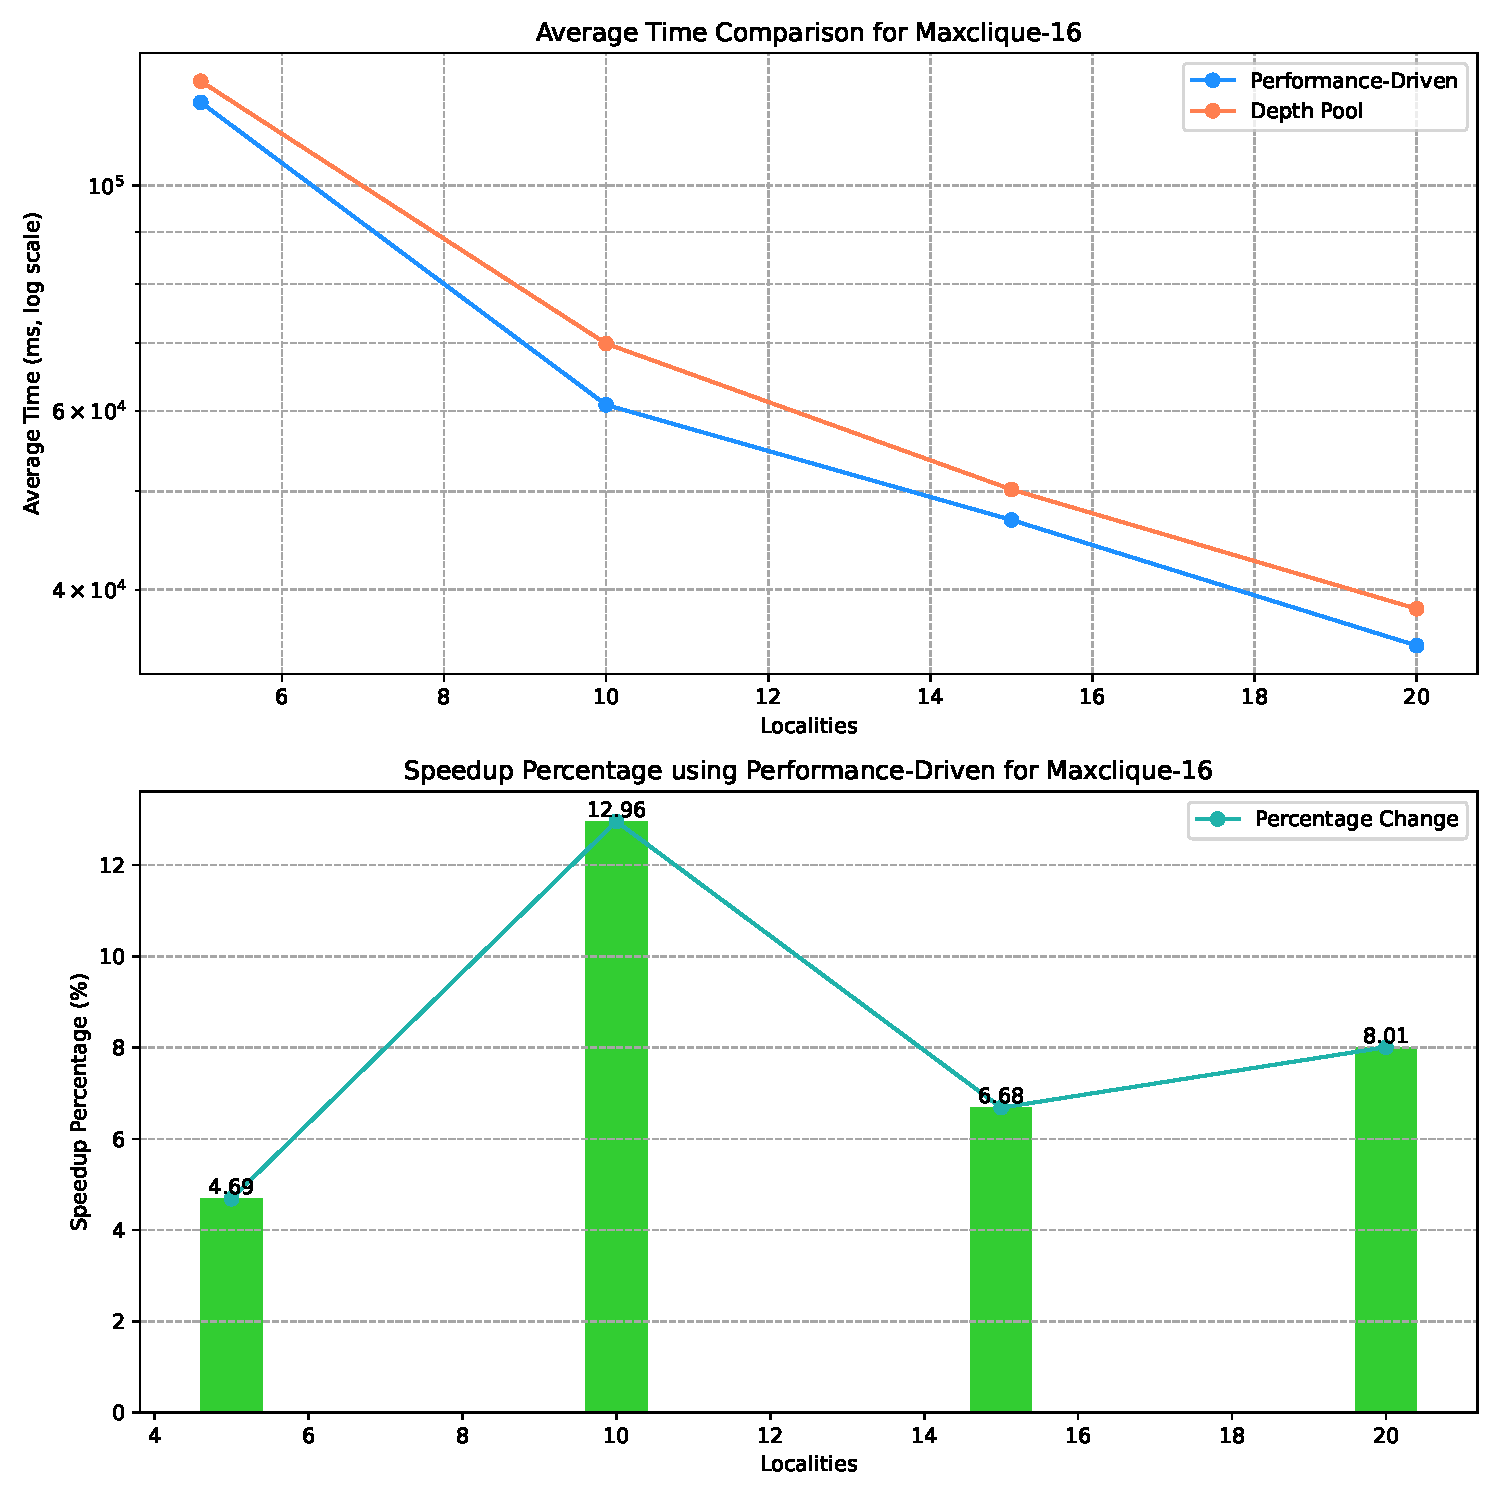
\includegraphics[width=0.9\textwidth]{images/time_comparison_max_simultaneously.pdf}
    \caption{simultaneous time comparison for Maxclique-16}
    \label{fig:time_comparison_max_simu}
\end{figure}
\FloatBarrier

It is evident that while Maxclique does exhibit significant super-linear slowdowns, under conditions of imbalanced node loads, the runtime advantages of the Maxclique application based on the Performance-Driven Workstealing Policy become more pronounced.
For instance, with a node count of 20, the speed improvement ratio escalates from 1.11\% during isolated execution to 8.01\% during simultaneous execution, an almost eight-fold increase.
This enhancement is presumably because, under imbalanced loads, the benefits from optimizing Workstealing targets significantly outweigh the costs introduced by additional tasks.
Furthermore, the graph indicates that, as the node count transitions from 10 to 15, the detrimental effects of additional tasks somewhat mitigate the speed improvements.
However, as the number of nodes continues to increase, the advantages of optimizing Workstealing targets gradually become more manifest.

\subsection{Simultaneous Performance Evaluation of NS-hivert}

For the NS-hivert program based on the Budget skeleton, the average results over ten runs for the runtime tests under simultaneous execution conditions are presented in \cref{fig:time_comparison_ns_simu}.
The evaluation encompasses both the runtime assessment and the comparison of speed improvement between the Performance-Driven Workstealing Policy and the original DepthPool Workstealing Policy.

\begin{figure}[h]
    \centering
    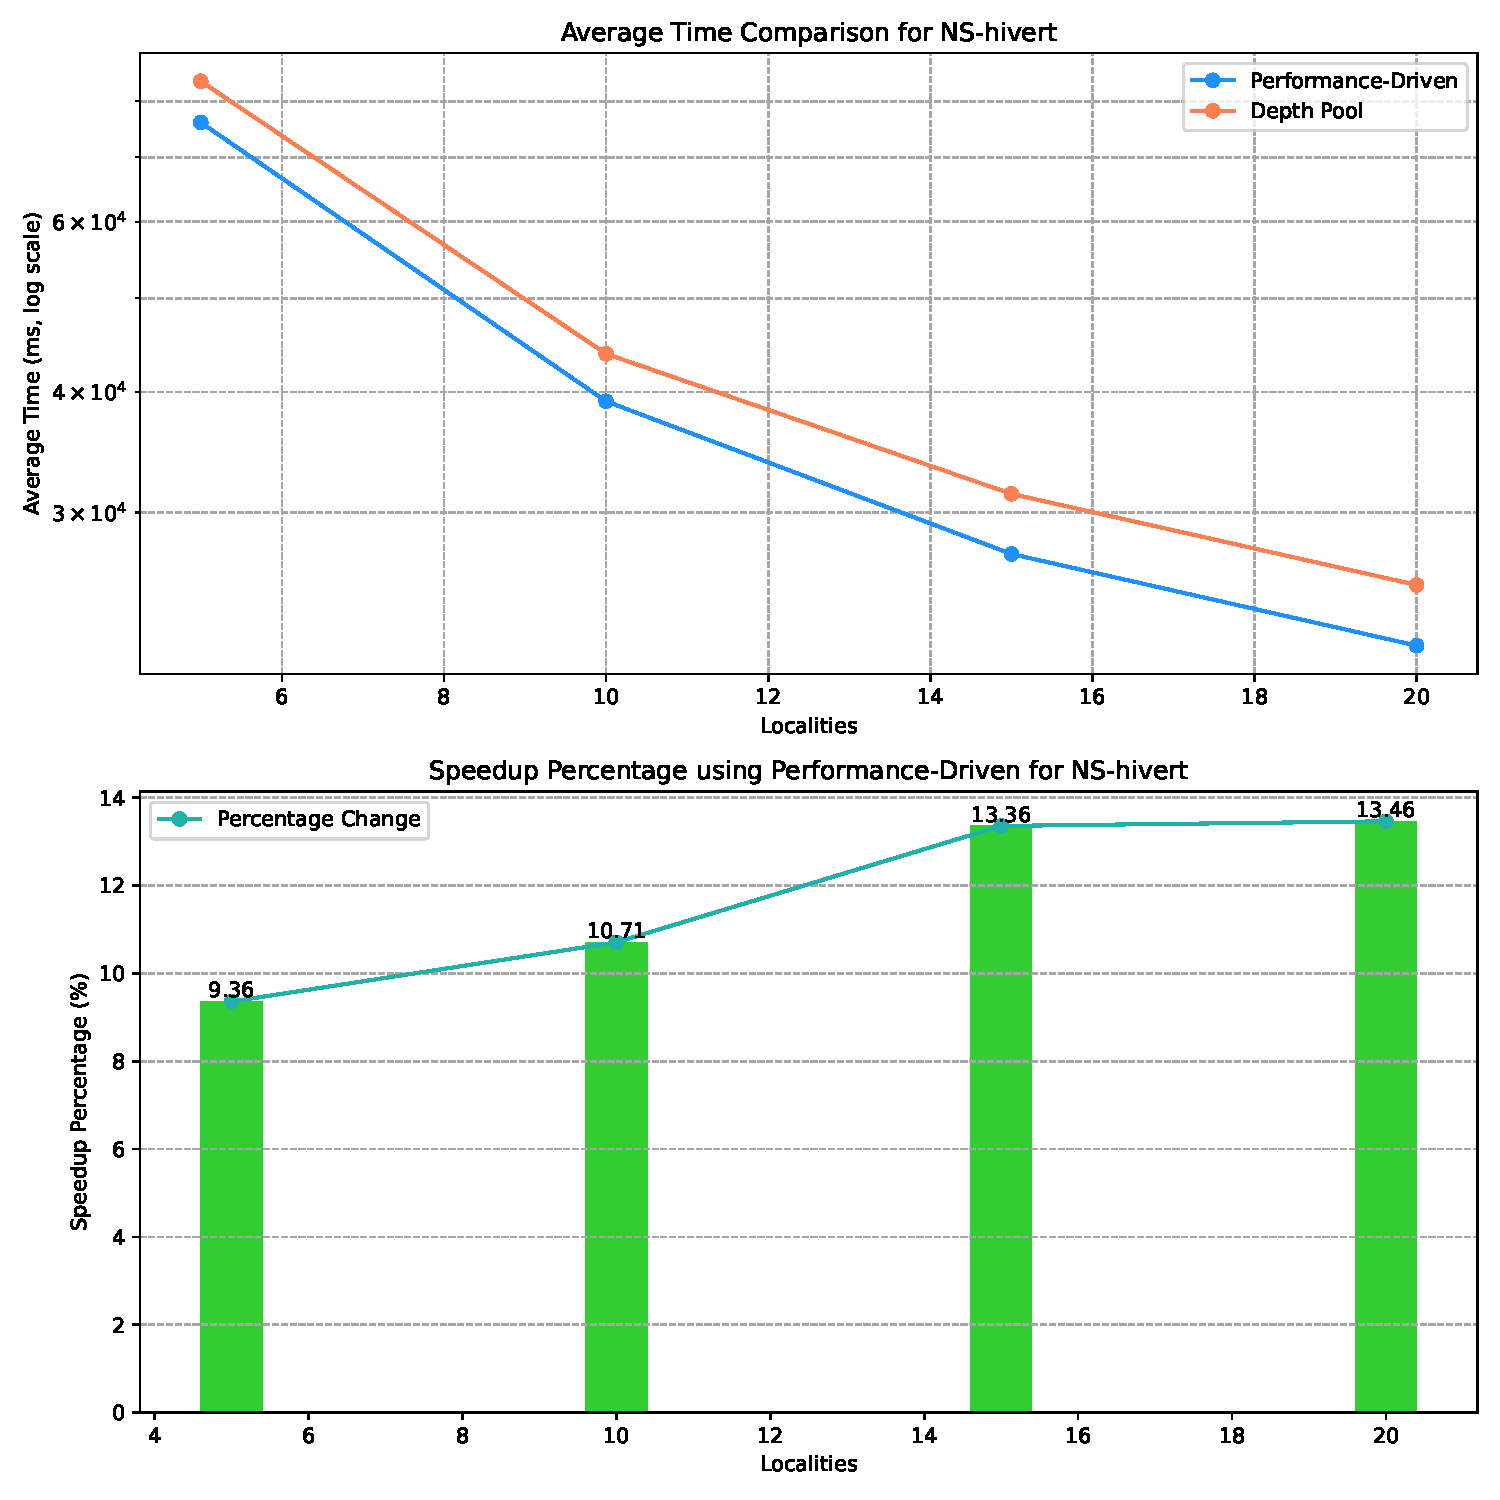
\includegraphics[width=0.9\textwidth]{images/time_comparison_ns_simultaneously.pdf}
    \caption{simultaneous time comparison for NS-hivert}
    \label{fig:time_comparison_ns_simu}
\end{figure}
\FloatBarrier

The graph reveals that within the NS-hivert program based on the Budget skeleton,
the performance enhancements from the Performance-Driven Workstealing Policy are considerably pronounced.
Starting from a 9.36\% improvement with 5 nodes, it steadily rises to 13.46\% with 20 nodes.
Given the limited optimization space that the Workstealing Policy has within the entire YewPar framework and the NS-hivert program,
achieving a 13.46\% performance boost is exceptionally commendable.

The modest increment observed in the graph from 15 to 20 nodes suggests that
as the number of nodes increases, the percentage of performance improvement brought by Workstealing is nearing its potential limit.
Most of the program's runtime is likely consumed by task processing and other overheads associated with the YewPar framework.

\section{Evaluation of Additional Performance Cost of Performance-driven Workstealing Policy Framework}

To investigate whether the lightweight design of the Performance-Driven Workstealing Policy incurs a significant additional performance overhead,
we compared the runtime of the NS-hivert application under different policies in a scenario where only one node with one worker (utilizing a single thread) was used.
We opted for the NS-hivert application due to its minimal runtime fluctuations, which minimizes interference.
To expedite the runtime for ease of measurement,
we adjusted its parameter \( g \) to \( g = 37 \) (genus: Depth in the tree to count until).

The test results are displayed in \cref{fig:time_comparison_ns_one_worker}.
\begin{figure}[h]
    \centering
    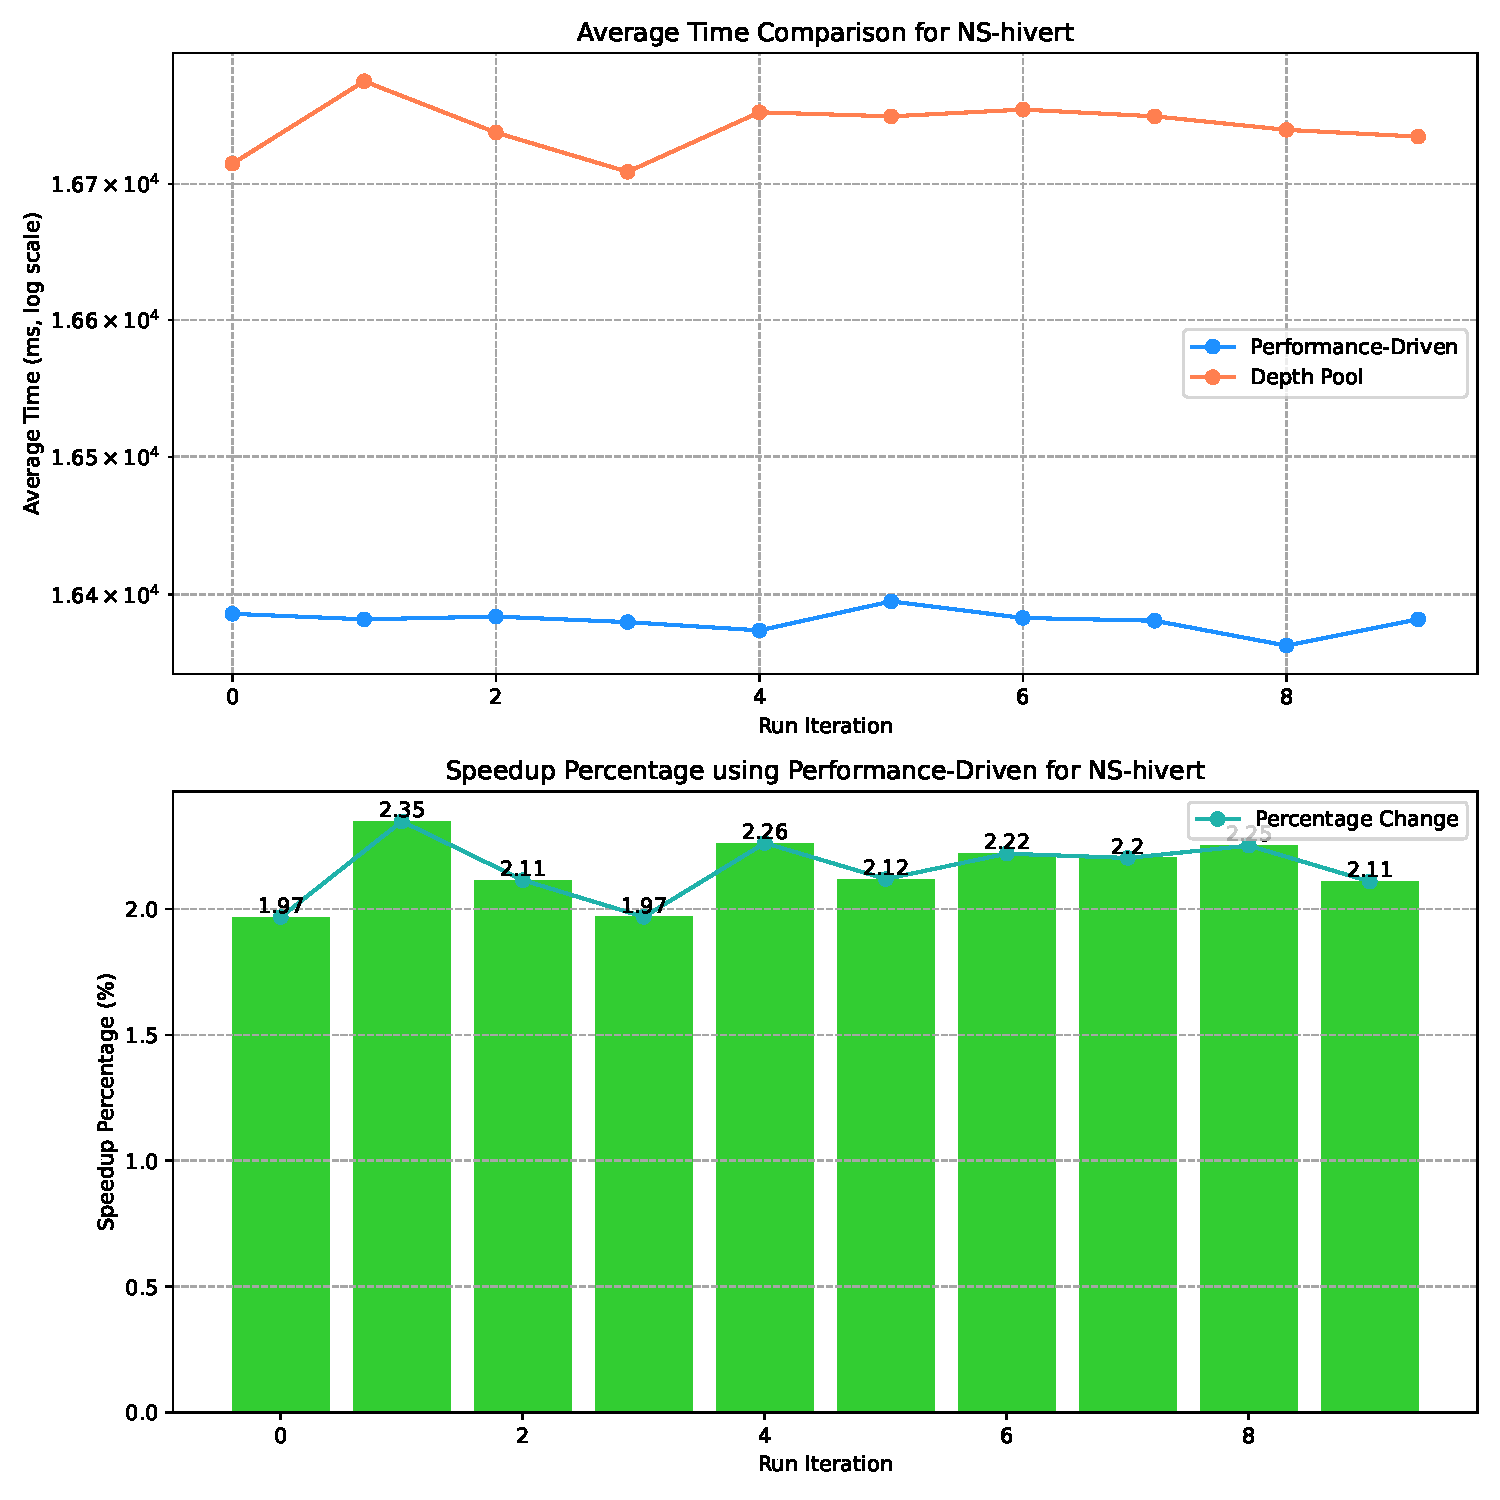
\includegraphics[width=0.9\textwidth]{images/time_comparison_ns_one_worker.pdf}
    \caption{time comparison for NS-hivert using one locality with one worker}
    \label{fig:time_comparison_ns_one_worker}
\end{figure}
\FloatBarrier

From the results, it is evident that due to the lightweight design of the Performance-Driven Workstealing Policy,
which incorporates mechanisms like lock-free operations to reduce additional computational overheads,
even when using a single worker (where no task stealing occurs, implying no optimization of stealing targets)
and in scenarios where the Performance-Driven Workstealing Policy dynamically refreshes stealing targets in the background,
it still achieves around a 2\% speed improvement over the original YewPar's Workstealing Policy.
This indicates the design's tremendous success in achieving its lightweight objective,
effectively reducing the performance losses introduced by the task-stealing framework.


%%%%%%%%%%%%%%%%%%%%%%%%%%%%%%%%%%%%%%%%%%%%%%%%%%%%%%%%%%%%%%%%%%%

\chapter{Future Work \& Conclusion}\label{conclusion}

\section{Future Work}

\subsection{Automatic Adjustment of Parameters}

In the previous \cref{design},
some fixed parameters in the algorithm, such as the proportion of historical data in the exponential smoothing algorithm,
were determined based on test results to be optimal values.
However, in more complex real-world scenarios,
these parameters might have better alternatives and present more room for optimization.
Hence, one could consider designing an algorithm that automatically adjusts these parameters
to ensure that all parameters within the Performance-Driven Workstealing Policy are always in an optimal state.

\subsection{Optimization for Performance Anomalies in Parallel Combined Searches}

From our previous evaluations, it was observed that under the Maxclique program,
the Performance-Driven Workstealing Policy frequently disrupted the heuristic search methods by frequently changing stealing targets,
jumbling the task execution sequence,
leading to the generation of more additional tasks for context speculation,
and subsequently slowing down the overall program execution speed.
It might be beneficial to design an algorithm that takes into account the preservation of task execution order when calculating stealing targets.
This might reduce the generation of extra tasks and further boost the program's execution speed in multi-node, multi-threaded scenarios.

\subsection{Substitute All YewPar Workstealing Policies}

Currently, the Performance-Driven Workstealing Policy has replaced policies in YewPar such as the DepthPool Policy,
thereby enhancing the performance of some of YewPar's skeletons.
However, due to time constraints, we have not yet attempted to replace policies like the Priority Ordered Policy.
As a result, not all skeletons in YewPar have benefited from the Performance-Driven Workstealing Policy.
This presents an avenue for future exploration and work.

\section{Conclusion}
Our objective was to enhance the performance of YewPar by refining its Workstealing strategy.
To this end, we devised and implemented a Performance-Driven Workstealing Policy,
which optimizes the stealing targets during Workstealing based on performance data from each node.
This involved the collection, processing, and transmission of performance data,
as well as calculations and caching for the optimal stealing targets,
complemented by a refreshing mechanism that offers two distinct methods.
Through optimization tailored for multi-threading and inter-node communication,
we achieved improvements in program execution speed at a minimal cost,
while maintaining excellent compatibility.

As per our evaluation results,
the Performance-Driven Workstealing Policy framework is lightweight, incurring minimal overheads.
Its optimization in the realm of Workstealing is remarkably evident.
In scenarios free of computational resource occupation,
the overall speed improvement of the program can surpass 8\%.
Moreover, in situations where node resources are unevenly utilized and there's contention,
speed enhancements can exceed 13\%.
Considering that these improvements were achieved merely by optimizing YewPar's Workstealing Policy,
and given that most of the program's runtime is spent processing tasks and generating new ones,
it's evident that adjusting the stealing targets based on the performance data of each node is a highly effective approach.
Therefore, the Performance-Driven Workstealing Policy stands out as an exceptional Workstealing strategy
and can seamlessly replace YewPar's original Workstealing Policy.


\appendix % first appendix
%%%%%%%%%%%%%%%%%%%%%%%%%%%%%%%%%%%%%%%%%%%%%%%%%%%%%%%%%%%%%%%%%%%
\chapter{Appendix}\label{appendix:link}

\section{Project description and Source code}\label{appendix:note}

The source code and other descriptions for this project can be found at :

\url{https://github.com/shadowxiehao/YewPar_with_PerformancePolicy}.

You can find specific instructions on the project such as installation instructions in the Readme file.

\section{Evaluation Data}\label{appendix:data}

The following data is the commands for evaluation and the 10 results(running time, Displayed by arrays, unit: ms) of running corresponding commands.
The commands should vary according to the actual environment.

\begin{lstlisting}

============================================================

Isolated evaluation:


Maxclique:
==========

mpiexec.openmpi -n 20 --host gpgnode-01,gpgnode-02,gpgnode-03,gpgnode-04,gpgnode-05,gpgnode-06,gpgnode-07,gpgnode-08,gpgnode-09,gpgnode-10,gpgnode-11,gpgnode-12,gpgnode-13,gpgnode-14,gpgnode-15,gpgnode-16,gpgnode-17,gpgnode-18,gpgnode-19,gpgnode-20 /cluster/gpg/hao/YewPar/build/install/bin/maxclique-16 -f /cluster/gpg/maxclique_instaces/brock800_2.clq --skeleton depthbounded -d 2 --hpx:threads 16

[14829,12791,16863,17266,16410,13920,14489,17646,21343,12549]

mpiexec.openmpi -n 20 --host gpgnode-01,gpgnode-02,gpgnode-03,gpgnode-04,gpgnode-05,gpgnode-06,gpgnode-07,gpgnode-08,gpgnode-09,gpgnode-10,gpgnode-11,gpgnode-12,gpgnode-13,gpgnode-14,gpgnode-15,gpgnode-16,gpgnode-17,gpgnode-18,gpgnode-19,gpgnode-20 /cluster/gpg/YewPar/build/install/bin/maxclique-16 -f /cluster/gpg/maxclique_instaces/brock800_2.clq --skeleton depthbounded -d 2 --hpx:threads 16

[16893,15822,17997,15739,16006,13570,17827,17189,16246,12595]

---

mpiexec.openmpi -n 15 --host gpgnode-01,gpgnode-02,gpgnode-03,gpgnode-04,gpgnode-05,gpgnode-06,gpgnode-07,gpgnode-08,gpgnode-09,gpgnode-10,gpgnode-11,gpgnode-12,gpgnode-13,gpgnode-14,gpgnode-15 /cluster/gpg/hao/YewPar/build/install/bin/maxclique-16 -f /cluster/gpg/maxclique_instaces/brock800_2.clq --skeleton depthbounded -d 2 --hpx:threads 16

[21533,19751,20677,25336,21294,25132,18389,17850,19703,16009]

mpiexec.openmpi -n 15 --host gpgnode-01,gpgnode-02,gpgnode-03,gpgnode-04,gpgnode-05,gpgnode-06,gpgnode-07,gpgnode-08,gpgnode-09,gpgnode-10,gpgnode-11,gpgnode-12,gpgnode-13,gpgnode-14,gpgnode-15 /cluster/gpg/YewPar/build/install/bin/maxclique-16 -f /cluster/gpg/maxclique_instaces/brock800_2.clq --skeleton depthbounded -d 2 --hpx:threads 16

[21678,22525,19146,18976,20766,22809,19951,20347,21012,19747]

---

---

mpiexec.openmpi -n 10 --host gpgnode-01,gpgnode-02,gpgnode-03,gpgnode-04,gpgnode-05,gpgnode-06,gpgnode-07,gpgnode-08,gpgnode-09,gpgnode-10 /cluster/gpg/hao/YewPar/build/install/bin/maxclique-16 -f /cluster/gpg/maxclique_instaces/brock800_2.clq --skeleton depthbounded -d 2 --hpx:threads 16

[24463,27543,25995,32465,32764,25782,27933,22756,32031,23569]

mpiexec.openmpi -n 10 --host gpgnode-01,gpgnode-02,gpgnode-03,gpgnode-04,gpgnode-05,gpgnode-06,gpgnode-07,gpgnode-08,gpgnode-09,gpgnode-10 /cluster/gpg/YewPar/build/install/bin/maxclique-16 -f /cluster/gpg/maxclique_instaces/brock800_2.clq --skeleton depthbounded -d 2 --hpx:threads 16

[29963,28186,28006,32229,27420,29927,29617,28761,28925,26073]

---

---

mpiexec.openmpi -n 5 --host gpgnode-01,gpgnode-02,gpgnode-03,gpgnode-04,gpgnode-05 /cluster/gpg/hao/YewPar/build/install/bin/maxclique-16 -f /cluster/gpg/maxclique_instaces/brock800_2.clq --skeleton depthbounded -d 2 --hpx:threads 16

[51414,64284,58569,66468,65849,55616,62883,64843,63617,60311]

mpiexec.openmpi -n 5 --host gpgnode-01,gpgnode-02,gpgnode-03,gpgnode-04,gpgnode-05 /cluster/gpg/YewPar/build/install/bin/maxclique-16 -f /cluster/gpg/maxclique_instaces/brock800_2.clq --skeleton depthbounded -d 2 --hpx:threads 16

[79945,50156,51396,53098,99086,99490,75471,51503,64685,68091]

---

==========

NS-hivert:

==========

---

mpiexec.openmpi -n 20 --host gpgnode-01,gpgnode-02,gpgnode-03,gpgnode-04,gpgnode-05,gpgnode-06,gpgnode-07,gpgnode-08,gpgnode-09,gpgnode-10,gpgnode-11,gpgnode-12,gpgnode-13,gpgnode-14,gpgnode-15,gpgnode-16,gpgnode-17,gpgnode-18,gpgnode-19,gpgnode-20 /cluster/gpg/hao/YewPar/build/install/bin/NS-hivert --skeleton budget -b 1000000 -g 47 --hpx:threads 16

[8942,9064,8978,8932,8904,8932,8966,9013,8956,8962]

mpiexec.openmpi -n 20 --host gpgnode-01,gpgnode-02,gpgnode-03,gpgnode-04,gpgnode-05,gpgnode-06,gpgnode-07,gpgnode-08,gpgnode-09,gpgnode-10,gpgnode-11,gpgnode-12,gpgnode-13,gpgnode-14,gpgnode-15,gpgnode-16,gpgnode-17,gpgnode-18,gpgnode-19,gpgnode-20 /cluster/gpg/YewPar/build/install/bin/NS-hivert --skeleton budget -b 1000000 -g 47 --hpx:threads 16

[9882,9948,9954,9978,9945,9989,9871,10042,10016,10056]

---

mpiexec.openmpi -n 15 --host gpgnode-01,gpgnode-02,gpgnode-03,gpgnode-04,gpgnode-05,gpgnode-06,gpgnode-07,gpgnode-08,gpgnode-09,gpgnode-10,gpgnode-11,gpgnode-12,gpgnode-13,gpgnode-14,gpgnode-15 /cluster/gpg/hao/YewPar/build/install/bin/NS-hivert --skeleton budget -b 1000000 -g 47 --hpx:threads 16

[11710,11826,11760,11772,11750,11760,11975,11757,11801,11746]

mpiexec.openmpi -n 15 --host gpgnode-01,gpgnode-02,gpgnode-03,gpgnode-04,gpgnode-05,gpgnode-06,gpgnode-07,gpgnode-08,gpgnode-09,gpgnode-10,gpgnode-11,gpgnode-12,gpgnode-13,gpgnode-14,gpgnode-15 /cluster/gpg/YewPar/build/install/bin/NS-hivert --skeleton budget -b 1000000 -g 47 --hpx:threads 16

[13005,13007,13054,13031,13051,13061,13039,12982,13024,13096]

---

mpiexec.openmpi -n 10 --host gpgnode-01,gpgnode-02,gpgnode-03,gpgnode-04,gpgnode-05,gpgnode-06,gpgnode-07,gpgnode-08,gpgnode-09,gpgnode-10 /cluster/gpg/hao/YewPar/build/install/bin/NS-hivert --skeleton budget -b 1000000 -g 47 --hpx:threads 16

[17445,17532,17515,17455,17486,17432,17525,17484,17506,17464]

mpiexec.openmpi -n 10 --host gpgnode-01,gpgnode-02,gpgnode-03,gpgnode-04,gpgnode-05,gpgnode-06,gpgnode-07,gpgnode-08,gpgnode-09,gpgnode-10 /cluster/gpg/YewPar/build/install/bin/NS-hivert --skeleton budget -b 1000000 -g 47 --hpx:threads 16

[19111,19149,19033,19113,19222,19072,19072,19023,19256,19037]

---

mpiexec.openmpi -n 5 --host gpgnode-01,gpgnode-02,gpgnode-03,gpgnode-04,gpgnode-05 /cluster/gpg/hao/YewPar/build/install/bin/NS-hivert --skeleton budget -b 1000000 -g 47 --hpx:threads 16

[34922,34849,34898,34913,34891,34926,34960,34891,34919,34859]

mpiexec.openmpi -n 5 --host gpgnode-01,gpgnode-02,gpgnode-03,gpgnode-04,gpgnode-05 /cluster/gpg/YewPar/build/install/bin/NS-hivert --skeleton budget -b 1000000 -g 47 --hpx:threads 16

[37633,37703,37710,37650,37613,37668,37720,37571,37682,37563]

---

==========

============================================================

Simultaneous evaluation:

Maxclique:
==========

mpiexec.openmpi -n 20 --host gpgnode-01,gpgnode-02,gpgnode-03,gpgnode-04,gpgnode-05,gpgnode-06,gpgnode-07,gpgnode-08,gpgnode-09,gpgnode-10,gpgnode-11,gpgnode-12,gpgnode-13,gpgnode-14,gpgnode-15,gpgnode-16,gpgnode-17,gpgnode-18,gpgnode-19,gpgnode-20 /cluster/gpg/hao/YewPar/build/install/bin/maxclique-16 -f /cluster/gpg/maxclique_instaces/brock800_2.clq --skeleton depthbounded -d 2 --hpx:threads 16

[29660,40314,37144,33314,37146,35187,39280,38449,30695,31253]

mpiexec.openmpi -n 20 --host gpgnode-01,gpgnode-02,gpgnode-03,gpgnode-04,gpgnode-05,gpgnode-06,gpgnode-07,gpgnode-08,gpgnode-09,gpgnode-10,gpgnode-11,gpgnode-12,gpgnode-13,gpgnode-14,gpgnode-15,gpgnode-16,gpgnode-17,gpgnode-18,gpgnode-19,gpgnode-20 /cluster/gpg/YewPar/build/install/bin/maxclique-16 -f /cluster/gpg/maxclique_instaces/brock800_2.clq --skeleton depthbounded -d 2 --hpx:threads 16

[34990,37954,42202,35970,39627,37308,47165,34588,36364,36959]

---

mpiexec.openmpi -n 15 --host gpgnode-01,gpgnode-02,gpgnode-03,gpgnode-04,gpgnode-05,gpgnode-06,gpgnode-07,gpgnode-08,gpgnode-09,gpgnode-10,gpgnode-11,gpgnode-12,gpgnode-13,gpgnode-14,gpgnode-15 /cluster/gpg/hao/YewPar/build/install/bin/maxclique-16 -f /cluster/gpg/maxclique_instaces/brock800_2.clq --skeleton depthbounded -d 2 --hpx:threads 16

[49062,45182,50122,40388,38596,53504,61126,34767,52585,43253]

mpiexec.openmpi -n 15 --host gpgnode-01,gpgnode-02,gpgnode-03,gpgnode-04,gpgnode-05,gpgnode-06,gpgnode-07,gpgnode-08,gpgnode-09,gpgnode-10,gpgnode-11,gpgnode-12,gpgnode-13,gpgnode-14,gpgnode-15 /cluster/gpg/YewPar/build/install/bin/maxclique-16 -f /cluster/gpg/maxclique_instaces/brock800_2.clq --skeleton depthbounded -d 2 --hpx:threads 16

[54296,57342,45869,52949,50054,51638,67120,37218,42635,43020]

---

---

mpiexec.openmpi -n 10 --host gpgnode-01,gpgnode-02,gpgnode-03,gpgnode-04,gpgnode-05,gpgnode-06,gpgnode-07,gpgnode-08,gpgnode-09,gpgnode-10 /cluster/gpg/hao/YewPar/build/install/bin/maxclique-16 -f /cluster/gpg/maxclique_instaces/brock800_2.clq --skeleton depthbounded -d 2 --hpx:threads 16

[66531,66494,60935,50364,56088,58545,60509,55681,63372,69744]

mpiexec.openmpi -n 10 --host gpgnode-01,gpgnode-02,gpgnode-03,gpgnode-04,gpgnode-05,gpgnode-06,gpgnode-07,gpgnode-08,gpgnode-09,gpgnode-10 /cluster/gpg/YewPar/build/install/bin/maxclique-16 -f /cluster/gpg/maxclique_instaces/brock800_2.clq --skeleton depthbounded -d 2 --hpx:threads 16

[62531,91967,80865,55159,56090,60476,77641,82621,61687,69789]

---

---

mpiexec.openmpi -n 5 --host gpgnode-01,gpgnode-02,gpgnode-03,gpgnode-04,gpgnode-05 /cluster/gpg/hao/YewPar/build/install/bin/maxclique-16 -f /cluster/gpg/maxclique_instaces/brock800_2.clq --skeleton depthbounded -d 2 --hpx:threads 16

[104810,106080,114325,127025,125424,119856,129894,121873,129900,128109]

mpiexec.openmpi -n 5 --host gpgnode-01,gpgnode-02,gpgnode-03,gpgnode-04,gpgnode-05 /cluster/gpg/YewPar/build/install/bin/maxclique-16 -f /cluster/gpg/maxclique_instaces/brock800_2.clq --skeleton depthbounded -d 2 --hpx:threads 16

[102019,158790,103343,130167,164195,114820,132898,108817,116030,135588]

---

==========

NS-hivert:

==========

mpiexec.openmpi -n 20 --host gpgnode-01,gpgnode-02,gpgnode-03,gpgnode-04,gpgnode-05,gpgnode-06,gpgnode-07,gpgnode-08,gpgnode-09,gpgnode-10,gpgnode-11,gpgnode-12,gpgnode-13,gpgnode-14,gpgnode-15,gpgnode-16,gpgnode-17,gpgnode-18,gpgnode-19,gpgnode-20 /cluster/gpg/hao/YewPar/build/install/bin/NS-hivert --skeleton budget -b 1000000 -g 47 --hpx:threads 16

[22083,22416,22299,20514,20333,22946,23012,21001,20655,23120]

mpiexec.openmpi -n 20 --host gpgnode-01,gpgnode-02,gpgnode-03,gpgnode-04,gpgnode-05,gpgnode-06,gpgnode-07,gpgnode-08,gpgnode-09,gpgnode-10,gpgnode-11,gpgnode-12,gpgnode-13,gpgnode-14,gpgnode-15,gpgnode-16,gpgnode-17,gpgnode-18,gpgnode-19,gpgnode-20 /cluster/gpg/YewPar/build/install/bin/NS-hivert --skeleton budget -b 1000000 -g 47 --hpx:threads 16

[25004,25496,25477,25484,24855,25586,25632,24856,24180,25778]

mpiexec.openmpi -n 15 --host gpgnode-01,gpgnode-02,gpgnode-03,gpgnode-04,gpgnode-05,gpgnode-06,gpgnode-07,gpgnode-08,gpgnode-09,gpgnode-10,gpgnode-11,gpgnode-12,gpgnode-13,gpgnode-14,gpgnode-15 /cluster/gpg/hao/YewPar/build/install/bin/NS-hivert --skeleton budget -b 1000000 -g 47 --hpx:threads 16

[26867,27067,28235,27508,25723,25471,28208,28128,26254,28272]

mpiexec.openmpi -n 15 --host gpgnode-01,gpgnode-02,gpgnode-03,gpgnode-04,gpgnode-05,gpgnode-06,gpgnode-07,gpgnode-08,gpgnode-09,gpgnode-10,gpgnode-11,gpgnode-12,gpgnode-13,gpgnode-14,gpgnode-15 /cluster/gpg/YewPar/build/install/bin/NS-hivert --skeleton budget -b 1000000 -g 47 --hpx:threads 16

[32329,31555,31457,30250,30670,30431,31528,31524,31236,32640]

mpiexec.openmpi -n 10 --host gpgnode-01,gpgnode-02,gpgnode-03,gpgnode-04,gpgnode-05,gpgnode-06,gpgnode-07,gpgnode-08,gpgnode-09,gpgnode-10 /cluster/gpg/hao/YewPar/build/install/bin/NS-hivert --skeleton budget -b 1000000 -g 47 --hpx:threads 16

[39736,37963,38072,40323,38470,39852,37845,40796,38552,39475]

mpiexec.openmpi -n 10 --host gpgnode-01,gpgnode-02,gpgnode-03,gpgnode-04,gpgnode-05,gpgnode-06,gpgnode-07,gpgnode-08,gpgnode-09,gpgnode-10 /cluster/gpg/YewPar/build/install/bin/NS-hivert --skeleton budget -b 1000000 -g 47 --hpx:threads 16

[44152,42980,44011,43471,43557,43119,44620,43576,45429,43059]

mpiexec.openmpi -n 5 --host gpgnode-01,gpgnode-02,gpgnode-03,gpgnode-04,gpgnode-05 /cluster/gpg/hao/YewPar/build/install/bin/NS-hivert --skeleton budget -b 1000000 -g 47 --hpx:threads 16

[75818,76999,76251,77031,75488,76587,76455,75528,75964,74382]

mpiexec.openmpi -n 5 --host gpgnode-01,gpgnode-02,gpgnode-03,gpgnode-04,gpgnode-05 /cluster/gpg/YewPar/build/install/bin/NS-hivert --skeleton budget -b 1000000 -g 47 --hpx:threads 16

[84444,82186,83962,84170,85396,81858,81957,85656,84645,84748]

==========


===========================================================

NS-hivert using only one thread:

/cluster/gpg/hao/YewPar/build/install/bin/NS-hivert --skeleton budget -b 1000000 -g 37 --hpx:threads 1

[16386,16382,16384,16380,16374,16395,16383,16381,16363,16382]

/cluster/gpg/YewPar/build/install/bin/NS-hivert --skeleton budget -b 1000000 -g 37 --hpx:threads 1

[16715,16776,16738,16709,16753,16750,16755,16750,16740,16735]

============================================================

\end{lstlisting}

% \chapter{Appendix second}


%%%%%%%%%%%%%%%%%%%%%%%%%%%%%%%%%%%%%%%%%%%%%%%%%%%%%%%%%%%%%%%%%%%
% \chapter{Second appendix}

%%%%%%%%%%%%%%%%%%%%%%%%%%%%%%%%%%%%%%%%%%%%%%%%%%%%%%%%%%%%%%%%%%%
% it is fine to change the bibliography style if you want
\bibliographystyle{plain}
\bibliography{mproj}
\end{document}
